\subsection{\texorpdfstring{The Grothendieck Group \(R_{K}(A)\)}{The Grothendieck Group R\_\{K\}(A)}}

Let \(\mathrm{K}\) be a commutative field and \(\mathrm{A}\) a \(\mathrm{K}\) -algebra. The set of classes of A-modules that are finite-dimensional vector spaces over \(\mathrm{K}\) is hereditary. The corresponding Grothendieck group is denoted by \(\mathrm{R}_{\mathrm{K}}(\mathrm{A})\) . It is a free \(\mathbf{Z}\) -module with basis the family \(([\mathrm{S}])_{\mathrm{S}\in \mathcal{S}}\) , where \(\mathcal{S}\) is the set of classes of simple A-modules that are finite-dimensional over \(\mathrm{K}\) . There exists a homomorphism

\[
\dim : \mathrm{R} _ {\mathrm{K}} (\mathrm{A}) \longrightarrow \mathbf {Z}
\]

characterized by \(\dim([E]) = [E : K]\) for every A-module E that is finite-dimensional over K. When A = K, it is an isomorphism. The submonoid of effective elements is denoted by \(\mathrm{R}_{\mathrm{K}}(\mathrm{A})^{+}\) .

Lemma 2. --- Let M and M' be A-modules that are finite-dimensional vector spaces over K. The supports (VIII, p.~190) of M and M' are disjoint if and only if there exists an \(a \in A\) such that \(a_{M} = 0_{M}\) and \(a_{M'} = 1_{M'}\) .

Suppose that there exists an \(a \in \mathrm{A}\) such that \(a_{\mathrm{M}} = 0_{\mathrm{M}}\) and \(a_{\mathrm{M}'} = 1_{\mathrm{M}'}\) . Let S be a simple A-module. If \(\operatorname{cl}(S)\) belongs to the support \(\mathcal{S}_{\mathrm{M}}\) of M, then the A-module S is isomorphic to one of the quotients of a Jordan-Hölder series of M and we have \(a_{\mathrm{S}} = 0_{\mathrm{S}}\) . Likewise, if \(\operatorname{cl}(S)\) belongs to the support \(\mathcal{S}_{\mathrm{M}'}\) of \(\mathrm{M}'\) , then we have \(a_{\mathrm{S}} = 1_{\mathrm{S}}\) . It follows that \(\mathcal{S}_{\mathrm{M}}\) and \(\mathcal{S}_{\mathrm{M}'}\) are disjoint.

Conversely, suppose that the sets \(S_{M}\) and \(S_{M'}\) are disjoint. They are finite because M and \(M'\) are finite-dimensional over K. Every simple A-module S whose class belongs to \(S_{M} \cup S_{M'}\) is finite-dimensional over K and a fortiori over the field \(\operatorname{End}_{\mathrm{A}}(\mathrm{S})\) . By Corollary 1 of Proposition 4 (VIII, p.~83), there exists an element \(b \in A\) such that we have \(b_{S} = 0_{S}\) (resp. \(b_{S} = 1_{S}\) ) for every simple A-module S whose class belongs to \(S_{M}\) (resp. \(S_{M'}\) ). Let \((\mathrm{M}_{i})_{0 \leqslant i \leqslant n}\) be a Jordan--Hölder series of M. By the above, we have \(bM_{i} \subset M_{i+1}\) for \(0 \leqslant i < n\) and therefore \((b^{n})_{\mathrm{M}} = 0_{\mathrm{M}}\) . The existence of a natural number m such that \(((1-b)^{m})_{\mathrm{M}^{\prime}}=0_{\mathrm{M}^{\prime}}\) is proved in the same way. Set \(\mathrm{P}(\mathrm{X})=1-(1-\mathrm{X}^{n})^{m}\) and \(a=\mathrm{P}(b)\) . The polynomial \(\mathrm{P}(\mathrm{X})\) is a multiple of \(X^{n}\) , so we have \(a_{M}=0_{M}\) , while the polynomial \(1-\mathrm{P}(\mathrm{X})\) is a multiple of \((1-\mathrm{X})^{m}\) , so we have \(a_{M^{\prime}}=1_{M^{\prime}}\) . This concludes the proof.

Let \(\mathrm{L}\) be an extension of \(\mathrm{K}\) . If \(\mathrm{M}\) is an A-module that is finite-dimensional over \(\mathrm{K}\) , then \(\mathrm{M}_{(\mathrm{L})}\) is an \(\mathrm{A}_{(\mathrm{L})}\) -module that is finite-dimensional over \(\mathrm{L}\) . Moreover, for every exact sequence

\[
0 \longrightarrow \mathrm{M} ^ {\prime} \longrightarrow \mathrm{M} \longrightarrow \mathrm{M} ^ {\prime \prime} \longrightarrow 0
\]

of A-modules, the sequence of \(A_{(L)}\) -modules

\[
0 \longrightarrow \mathrm{M} _ {(\mathrm{L})} ^ {\prime} \longrightarrow \mathrm{M} _ {(\mathrm{L})} \longrightarrow \mathrm{M} _ {(\mathrm{L})} ^ {\prime \prime} \longrightarrow 0
\]

deduced from it by extension of scalars is exact (II, §7, No.~7, p.~308, Proposition 14). Hence there exists a unique ring homomorphism \(u: \mathrm{R}_{\mathrm{K}}(\mathrm{A}) \to \mathrm{R}_{\mathrm{L}}(\mathrm{A}_{(\mathrm{L})})\) such that \(u([\mathrm{M}]) = [\mathrm{M}_{(\mathrm{L})}]\) for every A-module M that is finite-dimensional over K (No.~5).

THEOREM 1. --- The homomorphism \(u: \mathrm{R}_{\mathrm{K}}(\mathrm{A}) \to \mathrm{R}_{\mathrm{L}}(\mathrm{A}_{(\mathrm{L})})\) defined above is injective. Let \(\xi\) be an element of \(\mathrm{R}_{\mathrm{K}}(\mathrm{A})\) . Then \(\xi\) is effective if and only if \(u(\xi)\) is.

Lemma 3. --- Let S and T be two nonisomorphic simple A-modules that are finite-dimensional over K. The supports of the \(\mathrm{A}_{(\mathrm{L})}\) -modules \(\mathrm{S}_{(\mathrm{L})}\) and \(\mathrm{T}_{(\mathrm{L})}\) are disjoint.

By Lemma 2, there exists an element \(a \in \mathrm{A}\) such that \(a_{\mathrm{S}} = 0\) and \(a_{\mathrm{T}} = 1\) . The element \(1 \otimes a\) of \(\mathrm{A}_{(\mathrm{L})}\) acts as 0 on \(\mathrm{S}_{(\mathrm{L})}\) and as 1 on \(\mathrm{T}_{(\mathrm{L})}\) . By Lemma 2, the supports of the \(\mathrm{A}_{(\mathrm{L})}\) -modules \(\mathrm{S}_{(\mathrm{L})}\) and \(\mathrm{T}_{(\mathrm{L})}\) are disjoint.

Let us prove Theorem 1. Let S be the set of classes of simple A-modules that are finite-dimensional over K. The family \(([S])_{S \in \mathcal{S}}\) is a basis of the Z-module \(R_{K}(A)\) . Let \(S \in S\) . The \(A_{(L)}\) -module \(S_{(L)}\) is not zero, so its support is not empty. Let \(S'\) be an element of this support. By Lemma 1 of VIII, p.~190, there exists a homomorphism \(f_{S'} : R_L(A_{(L)}) \to Z\) such that \(f_{S'}([E]) = \ell_{S'}(E)\) for every \(A_{(L)}\) -module E that is finite-dimensional over L. We have \(f_{S'}([S_{(L)}]) \neq 0\) by construction and \(f([T_{(L)}]) = 0\) for every \(T \in S - \{S\}\) by Lemma 3. We have therefore proved that the elements of \(R_L(A_{(L)})\) of the form \([S_{(L)}]\) for \(S \in S\) are linearly independent over Z. It follows that the homomorphism u is injective.

Let \(S \in \mathscr{S}\) , and let \(S'\) be an element of the support of \(S_{(L)}\) . For every \(\xi \in R_K(A)\) , the coordinate of \(\xi\) of index {[}S{]} in the basis \(([S])_{S \in \mathscr{S}}\) is \(f_{S'}(u(\xi)) / [S_{(L)} : S']\) . It follows that if \(u(\xi)\) is effective, then so is \(\xi\) .

\subsection{Multiplicative Structure on K(C)}

Let K be a commutative ring and A a bigebra over the ring K (III, §11, No.~4, p.~585), with coproduct c and counit \(\gamma\) . Unless stated otherwise, the tensor products are over K. Let E and F be (left) A-modules. The tensor product \(E \otimes F\) is endowed with an \((A \otimes A)\) -module structure characterized by the formula

\[
(a \otimes b) (x \otimes y) = a x \otimes b y\tag{11}
\]

for \(a, b \in \mathrm{A}\) , \(x \in \mathrm{E}\) , and \(y \in \mathrm{F}\) . Using the homomorphism \(c: \mathrm{A} \to \mathrm{A} \otimes \mathrm{A}\) , we deduce from this \((\mathrm{A} \otimes \mathrm{A})\) -module an A-module \(c_*(\mathrm{E} \otimes \mathrm{F})\) (II, §1, No.~13, p.~221). More precisely, let \(a \in \mathrm{A}\) ; if \(c(a) = \sum_{i} a_{i} \otimes b_{i}\) , then we have

\[
a (x \otimes y) = \sum_ {i} a _ {i} x \otimes b _ {i} y\tag{12}
\]

for \(x \in E\) and \(y \in F\) . By abuse of notation, we also denote the resulting A-module by \(E \otimes F\) . It follows immediately from the coassociativity of c that the canonical isomorphism of K-modules

\[
\varphi : (\mathrm{E} \otimes \mathrm{F}) \otimes \mathrm{G} \longrightarrow \mathrm{E} \otimes (\mathrm{F} \otimes \mathrm{G})
\]

is A-linear for all A-modules E, F, and G. Likewise, if the bigebra A is cocommutative, then the canonical isomorphism from \(E \otimes F\) to \(F \otimes E\) is A-linear. Finally, let \(K_{\gamma}\) be the A-module with underlying group K and external law \((a, x) \mapsto \gamma(a)x\) . The canonical isomorphism from \(K \otimes E\) (resp. \(E \otimes K\) ) to E is an isomorphism of A-modules from \(K_{\gamma} \otimes E\) (resp. \(E \otimes K_{\gamma}\) ) to E.

PROPOSITION 9. --- Let K be a commutative ring, A a bigebra over K with counit γ, and C an additive set of classes of A-modules with the following properties:

\begin{enumerate}
\def\labelenumi{(\roman{enumi})}
\item
  Every A-module of type \(\mathcal{C}\) is a projective (* or, more generally, flat*) K-module.
\item
  If the A-modules E and F are of type C, then so is the A-module \(E \otimes F\) .
\item
  The A-module \(\mathrm{K}_{\gamma}\) defined above is of type \(\mathcal{C}\) .
\end{enumerate}

Then there exists a unique ring structure on the additive group \(\mathrm{K}(\mathcal{C})\) whose multiplication satisfies

\[
[ \mathrm{E} ] _ {\mathcal {C}} [ \mathrm{F} ] _ {\mathcal {C}} = [ \mathrm{E} \otimes \mathrm{F} ] _ {\mathcal {C}}
\]

for all A-modules E and F of type C. The unit element of \(\mathrm{K}(\mathcal{C})\) is \([\mathrm{K}_{\gamma}]_{\mathcal{C}}\) . If the bigebra A is cocommutative, then the ring \(\mathrm{K}(\mathcal{C})\) is commutative.

Endowed with the law of composition given by \((\mathrm{E},\mathrm{F})\mapsto\mathrm{cl}(\mathrm{E}\otimes\mathrm{F})\) , the set C is a monoid with unit element \(\mathrm{cl}(\mathrm{K}_{\gamma})\) . Consequently, \(Z^{(\mathcal{C})}\) is canonically endowed with the structure of a ring with multiplication characterized by the formula

\[
\operatorname{cl} (\mathrm{E}) \operatorname{cl} (\mathrm{F}) = \operatorname{cl} (\mathrm{E} \otimes \mathrm{F})\tag{13}
\]

and unit element \(\operatorname{cl}(\mathrm{K}_{\gamma})\) (III, §2, No.~6, p.~446).

Given an A-module F of type C and an exact sequence

\[
0 \longrightarrow \mathrm{E} ^ {\prime} \longrightarrow \mathrm{E} \longrightarrow \mathrm{E} ^ {\prime \prime} \longrightarrow 0\tag{\( \mathcal{E} \)}
\]

of A-modules of type C, the sequence

\[
0 \longrightarrow \mathrm{E} ^ {\prime} \otimes \mathrm{F} \longrightarrow \mathrm{E} \otimes \mathrm{F} \longrightarrow \mathrm{E} ^ {\prime \prime} \otimes \mathrm{F} \longrightarrow 0\tag{\(\left(\mathcal{E}\otimes \mathrm{F}\right)\)}
\]

deduced from \((\mathcal{E})\) is exact because F is projective ( \(^{*}\) or, more generally, flat \(_{*}\) ) over K (II, §3, No.~6, p.~251, Proposition 5 and II, §3, No.~7, p.~257, Corollary 6). In the notation of No.~2, we then have

\[
r _ {\mathcal {E} \otimes \mathrm{F}} = r _ {\mathcal {E}} \operatorname{cl} (\mathrm{F}).\tag{14}
\]

It follows that the subgroup R of \(\mathbf{Z}^{(\mathcal{C})}\) generated by the elements of the form \(r_{\mathcal{E}}\) is a right ideal of the ring \(\mathbf{Z}^{(\mathcal{C})}\) , and one proves likewise that it is a left ideal of \(\mathbf{Z}^{(\mathcal{C})}\) . By definition, \(\mathrm{K}(\mathcal{C})\) is the quotient group \(\mathbf{Z}^{(\mathcal{C})}/\mathrm{R}\) ; hence there exists a unique ring structure on \(\mathrm{K}(\mathcal{C})\) whose multiplication satisfies \([E]_{\mathcal{C}}[F]_{\mathcal{C}} = [E \otimes F]_{\mathcal{C}}\) for all A-modules E and F of type C. Its unit element is \([K_{\gamma}]\) .

When the bigebra A is cocommutative, the monoid C is commutative; it follows that the ring \(\mathbf{Z}^{(\mathcal{C})}\) and the quotient ring \(\mathrm{K}(\mathcal{C})\) are commutative.

Remark. --- Under only assumptions (i) and (ii) of Proposition 9, the Grothendieck group \(\mathrm{K}^{\prime}(\mathcal{C})\) for direct sums (VIII, p.~188) has a unique ring structure whose multiplication satisfies \([E]_{\mathcal{C}}^{\prime}[F]_{\mathcal{C}}^{\prime} = [E \otimes F]_{\mathcal{C}}^{\prime}\) . Its unit element is \([K_{\gamma}]_{\mathcal{C}}^{\prime}\) . The ring \(\mathrm{K}^{\prime}(\mathcal{C})\) is commutative if the bigebra A is cocommutative. The proof is analogous to that of Proposition 9 because the group \(\mathrm{K}^{\prime}(\mathcal{C})\) can be identified with \(\mathbf{Z}^{(\mathcal{C})}/\mathrm{R}^{\prime}\) , where \(R^{\prime}\) is the subgroup of \(\mathbf{Z}^{(\mathcal{C})}\) generated by the elements of the form \(\mathrm{cl}(\mathrm{E}^{\prime} \oplus \mathrm{E}^{\prime\prime}) - \mathrm{cl}(\mathrm{E}^{\prime}) - \mathrm{cl}(\mathrm{E}^{\prime\prime})\) (loc. cit.).

Under assumptions (i), (ii), and (iii) of Proposition 9, the ring \(\mathrm{K}(\mathcal{C})\) is called the Grothendieck ring of C. These conditions are, in particular, satisfied when K is a field and C is the set of classes of A-modules that are finite-dimensional over K. Consequently, we have the following.

COROLLARY. --- Let A be a bigebra with counit \(\gamma\) over a commutative field K. Then there exists a unique ring structure on the additive group \(\mathrm{R}_{\mathrm{K}}(\mathrm{A})\) whose multiplication satisfies

\[
[ \mathrm{E} ] _ {\mathcal {C}} [ \mathrm{F} ] _ {\mathcal {C}} = [ \mathrm{E} \otimes_ {\mathrm{K}} \mathrm{F} ] _ {\mathcal {C}}
\]

for all A-modules E and F that are finite-dimensional over K. The unit element of \(\mathrm{R}_{\mathrm{K}}(\mathrm{A})\) is \([\mathrm{K}_{\gamma}]_{\mathcal{C}}\) . If the bigebra A is cocommutative, then the ring \(\mathrm{R}_{\mathrm{K}}(\mathrm{A})\) is commutative.

Examples. --- 1) Let K be a commutative field. Let G be a group, and let K{[}G{]} be the algebra of the group G. We identify G with its canonical image in K{[}G{]} (III, §2, No.~6, p.~446).

We endow K{[}G{]} with the structure of a bigebra with coproduct c and counit \(\gamma\) given by

\[
c (g) = g \otimes g, \quad \gamma (g) = 1 \quad (g \in G).\tag{15}
\]

Let \(\mathrm{E}\) and \(\mathrm{F}\) be \(\mathrm{K}[\mathrm{G}]\) -modules; by formula (12), the \(\mathrm{K}[\mathrm{G}]\) -module structure on \(\mathrm{E} \otimes \mathrm{F}\) is given by

\[
g (x \otimes y) = g x \otimes g y \quad (g \in \mathrm{G}, x \in \mathrm{E}, y \in \mathrm{F}).\tag{16}
\]

The K{[}G{]}-module \(K_{\gamma}\) is the vector space K endowed with the action of G defined by \(g\lambda = \lambda\) for \(g \in G\) and \(\lambda \in K\) .

The ring \(\mathrm{R}_{\mathrm{K}}(\mathrm{K}[\mathrm{G}])\) is also denoted by \(\mathrm{R}_{\mathrm{K}}(\mathrm{G})\) . It is commutative; its multiplication is given by {[}E{]} {[}F{]} = {[}E \(\otimes_{\mathrm{K}}\) F{]}, and the unit element of \(\mathrm{R}_{\mathrm{K}}(\mathrm{G})\) is \([K_{\gamma}]\) .

*2) Let \(\mathfrak{g}\) be a Lie algebra over a commutative field \(K\) and \(U(\mathfrak{g})\) its enveloping algebra; we identify \(\mathfrak{g}\) with its canonical image in \(U(\mathfrak{g})\) (Lie, I, §2, No.~7, p.~39, Corollary 2). We endow \(U(\mathfrak{g})\) with the structure of a bigebra with coproduct \(c\) and counit \(\gamma\) given by

\[
c (\xi) = \xi \otimes 1 + 1 \otimes \xi , \quad \gamma (\xi) = 0\tag{17}
\]

for \(\xi\in\mathfrak{g}\) (Lie, II, §1, No.~4, p.~115).

Let \(\mathrm{E}\) and \(\mathrm{F}\) be \(\mathrm{U}(\mathfrak{g})\) -modules; by formula (17), the \(\mathrm{U}(\mathfrak{g})\) -module structure on \(\mathrm{E} \otimes \mathrm{F}\) is characterized by

\[
\xi (x \otimes y) = \xi x \otimes y + x \otimes \xi y\tag{18}
\]

for \(\xi\in\mathfrak{g}, x\in\mathrm{E}\) , and \(y\in\mathrm{F}\) .

The Grothendieck ring \(\mathrm{R}_{\mathrm{K}}(\mathrm{U}(\mathfrak{g}))\) is also denoted by \(\mathcal{R}(\mathfrak{g})\) in Lie, VIII, §7, No.~6, p.~139.*

Let A be a commutative ring. We can view A as a bigebra that is cocommutative over itself, with coproduct the natural isomorphism from A to \(A \otimes_{A} A\) and counit \(Id_{A}\) (III, §11, No.~4, p.~585). By Proposition 9, we obtain the following result.

PROPOSITION 10. --- Let A be a commutative ring, and let C be an additive set of classes of A-modules satisfying the following three conditions:

\begin{enumerate}
\def\labelenumi{(\roman{enumi})}
\item
  Every A-module of type \(\mathcal{C}\) is projective (* or, more generally, flat*)
\item
  If \(\mathrm{E}\) and \(\mathrm{F}\) are A-modules of type \(\mathcal{C}\) , then the A-module \(\mathrm{E} \otimes_{\mathrm{A}} \mathrm{F}\) is also of type \(\mathcal{C}\) .
\item
  The A-module A is of type \(\mathcal{C}\) .
\end{enumerate}

Then there exists a unique ring structure on the additive group \(\mathrm{K}(\mathcal{C})\) satisfying \([E]_{\mathcal{C}}[F]_{\mathcal{C}} = [E \otimes_{A} F]_{\mathcal{C}}\) for every pair E, F of A-modules of type C. The unit element of \(\mathrm{K}(\mathcal{C})\) is \([A]_{\mathcal{C}}\) .

\subsection{\texorpdfstring{The Grothendieck Group \(K_{0}(A)\)}{The Grothendieck Group K\_\{0\}(A)}}

Let \(\mathrm{A}\) be a ring. The set \(\mathcal{P}(\mathrm{A})\) of classes of finitely generated projective A-modules is additive; we denote the Grothendieck group \(\mathrm{K}(\mathcal{P}(\mathrm{A}))\) by \(\mathrm{K}_0(\mathrm{A})\) .

For the law of composition \((\mathrm{E},\mathrm{E}^{\prime})\mapsto\mathrm{cl}(\mathrm{E}\oplus\mathrm{E}^{\prime})\) , the set \(\mathcal{P}(\mathrm{A})\) is a commutative monoid. Moreover, every exact sequence of projective A-modules

\[
0 \longrightarrow \mathrm{E} ^ {\prime} \longrightarrow \mathrm{E} \longrightarrow \mathrm{E} ^ {\prime \prime} \longrightarrow 0
\]

splits (II, §2, No.~2, p.~231, Proposition 4), so that E is isomorphic to \(E^{\prime} \oplus E^{\prime\prime}\) . The mapping \(E \mapsto [E]\) from \(\mathcal{P}(A)\) to \(K_{0}(A)\) therefore defines an isomorphism from the group of differences of the monoid \(\mathcal{P}(A)\) to \(K_{0}(A)\) (VIII, p.~188).

For every finitely generated projective module P, there exists a finitely generated projective module \(P'\) such that \(P \oplus P'\) is free (II, §2, No.~2, p.~232, Corollary 1). Let E and F be finitely generated projective A-modules; by I, §2, No.~4, p.~18, Proposition 6, we have \([E] = [F]\) in \(K_{0}(A)\) if and only if there exists a finitely generated free A-module L such that the A-modules \(E \oplus L\) and \(F \oplus L\) are isomorphic. We then say that E and F are stably isomorphic;

this does not necessarily imply that E and F are isomorphic (VIII, p.~207, Exercise 2 and VIII, p.~210, Exercise 14).

When the ring A is commutative, there exists a commutative ring structure on the additive group \(K_{0}(A)\) whose multiplication is characterized by the formula \([\mathrm{E}]_{\mathcal{P}(\mathrm{A})}[\mathrm{F}]_{\mathcal{P}(\mathrm{A})} = [\mathrm{E} \otimes_{\mathrm{A}} \mathrm{F}]_{\mathcal{P}(\mathrm{A})}\) (VIII, p.~199, Proposition 10).

Remark. --- Let A be a semisimple ring. Every A-module is then semisimple and projective (VIII, p.~138, Proposition 4); we therefore have the equality

\[
\mathscr {L} \mathscr {F} (\mathrm{A}) = \mathscr {S S} (\mathrm{A}) = \mathscr {P} (\mathrm{A})
\]

(cf.~No.~4 for the definitions of \(\mathcal{LF}(\mathrm{A})\) and \(\mathcal{SS}(\mathrm{A})\) ). We therefore have \(\mathrm{K}_0(\mathrm{A}) = \mathrm{R}(\mathrm{A})\) by the definitions of these Grothendieck groups.

Example. --- If every finitely generated projective A-module is free, then the rank defines an isomorphism from \(K_{0}(A)\) to Z. This is, in particular, the case when A is a principal ideal domain (VII, §1, No.~3, p.~15, Corollary 3) or when A is a local ring (VIII, p.~36, Corollary 6).

\subsection{\texorpdfstring{The Grothendieck Group \(K_{0}(A)\) of an Artinian Ring}{The Grothendieck Group K\_\{0\}(A) of an Artinian Ring}}

Let A be a left Artinian ring. Let r be its radical; it is a nilpotent two-sided ideal of A, and the ring A/r is semisimple (VIII, p.~173, Proposition 1). By the corollary of VIII, p.~176, the mapping P \(\mapsto\) cl(P/rP) is an isomorphism from the monoid \(\mathcal{P}(A)\) to the monoid \(\mathcal{P}(A/r)\) . We deduce from it a group isomorphism \(\gamma\) from \(K_{0}(A)\) to \(K_{0}(A/r)\) characterized by the relation \(\gamma([\mathrm{P}]_{\mathcal{P}(A)}) = [\mathrm{P}/\mathfrak{r}\mathrm{P}]_{\mathcal{P}(A/r)}\) for every finitely generated projective A-module P.

Since the ring A/r is semisimple, the remark above implies the equality \(\mathrm{R}(\mathrm{A}/\mathfrak{r}) = \mathrm{K}_{0}(\mathrm{A}/\mathfrak{r})\) . The modules of finite length over the ring A/r are simply the semisimple modules of finite length over the ring A (VIII, p.~174, Proposition 2); consequently, we can identify \(\mathcal{L}\mathcal{F}(\mathrm{A}/\mathfrak{r})\) with \(\mathcal{S}\mathcal{S}(\mathrm{A})\) and \(\mathrm{R}(\mathrm{A}/\mathfrak{r})\) with \(\mathrm{K}(\mathcal{S}\mathcal{S}(\mathrm{A}))\) . We denote by \(\delta\) the homomorphism \(\gamma_{\mathcal{L}\mathcal{F}(\mathrm{A}),\mathcal{S}\mathcal{S}(\mathrm{A})}\) from \(\mathrm{R}(\mathrm{A}/\mathfrak{r}) = \mathrm{K}(\mathcal{S}\mathcal{S}(\mathrm{A}))\) to \(\mathrm{R}(\mathrm{A}) = \mathrm{K}(\mathcal{L}\mathcal{F}(\mathrm{A}))\) (VIII, p.~191, Remark 1); it is an isomorphism. Finally, we have \(\mathcal{P}(\mathrm{A}) \subset \mathcal{L}\mathcal{F}(\mathrm{A})\) , and we set \(\varepsilon =\) \(\gamma_{\mathcal{L}\mathcal{F}(\mathrm{A}),\mathcal{P}(\mathrm{A})}\) . We have defined a diagram

\pandocbounded{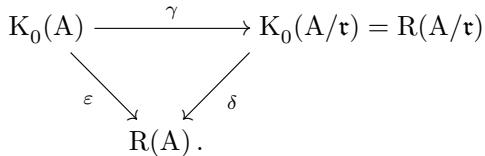
\includegraphics[keepaspectratio]{images/part002_05770a86.jpg}}

We denote the (finite) set of classes of simple A-modules by \(\mathcal{S}\) ; for every \(\lambda \in \mathcal{S}\) , choose a module \(S_{\lambda}\) of class \(\lambda\) and a projective cover \((P_{\lambda}, u_{\lambda})\) of \(S_{\lambda}\) (VIII, p.~175, Proposition 4). It follows from Proposition 6 of VIII, p.~176 that \(K_0(A)\) is a free \(\mathbf{Z}\) -module with basis the family \(([P_{\lambda}]_{\mathcal{P}(A)})_{\lambda \in \mathcal{S}}\) . Moreover, since \(S_{\lambda}\) is isomorphic to \(P_{\lambda} / \mathfrak{r}P_{\lambda}\) (VIII, p.~176), \(\gamma\) transforms the basis \(([P_{\lambda}]_{\mathcal{P}(A)})_{\lambda \in \mathcal{S}}\) of \(K_0(A)\) into the basis \(([S_{\lambda}])_{\lambda \in \mathcal{S}}\) of \(R(A / \mathfrak{r})\) . The isomorphism \(\delta\) transforms the basis \(([S_{\lambda}])_{\lambda \in \mathcal{S}}\) of \(R(A / \mathfrak{r})\) into the basis \(([S_{\lambda}])_{\lambda \in \mathcal{S}}\) of \(R(A)\) .

The Cartan matrix of A is the matrix \((a_{\lambda\mu})\) of the homomorphism of Z-modules \(\varepsilon: K_{0}(A) \to R(A)\) with respect to bases \(([P_{\lambda}]_{\mathcal{P}(A)})_{\lambda \in \mathcal{S}}\) of \(K_{0}(A)\) and \(([S_{\lambda}])_{\lambda \in \mathcal{S}}\) of \(R(A)\) . By definition, we have

\[
[ \mathrm{P} _ {\mu} ] = \sum_ {\lambda \in \mathcal {S}} a _ {\lambda \mu} [ \mathrm{S} _ {\lambda} ] \quad (\mu \in \mathcal {S})\tag{19}
\]

in the group R(A). In other words, \(a_{\lambda\mu}\) is the number of quotients isomorphic to \(S_{\lambda}\) in a Jordan--Hölder series of the A-module \(P_{\mu}\) .

Set \(\pi = \varepsilon \circ \gamma^{-1} \circ \delta^{-1}\) ; it is an endomorphism of the group R(A). If M is a finitely generated semisimple A-module and (P, \(u\) ) a projective cover of M, then we have \(\pi([M]) = [P]\) . By formula (19), the matrix of \(\pi\) with respect to the basis \(([S_{\lambda}])_{\lambda \in \mathcal{S}}\) of R(A) is simply the Cartan matrix of A.

\subsection{\texorpdfstring{Change of Rings for \(K_{0}(A)\)}{Change of Rings for K\_\{0\}(A)}}

Let A and B be rings. Let \(f: A \to B\) be a ring homomorphism. If P is a finitely generated projective A-module, then the B-module \(f^{*}(P) = B \otimes_{A} P\) is projective and finitely generated (II, §5, No.~2, p.~281, Corollary). The mapping \(P \mapsto \text{cl}(f^{*}(P))\) is a homomorphism from the monoid \(\mathcal{P}(A)\) to the monoid \(\mathcal{P}(B)\) and therefore defines a homomorphism \(f^{*}: K_{0}(A) \to K_{0}(B)\) characterized by the relation \(f^{*}([P]_{\mathcal{P}(A)}) = [f^{*}(P)]_{\mathcal{P}(B)}\) for every finitely generated projective A-module P. If \(g: B \to C\) is a second ring homomorphism, then it follows from the transitivity of the extension of scalars (II, §5, No.~1, p.~278, Proposition 2) that the homomorphisms \((g \circ f)^*\) and \(g^{*} \circ f^{*}\) from \(\mathrm{K}_{0}(\mathrm{A})\) to \(\mathrm{K}_{0}(\mathrm{C})\) are equal.

Suppose that \(f\) makes B into a finitely generated projective left A-module. Let Q be a finitely generated projective left B-module. Then Q is a direct factor of a finitely generated free B-module that is projective and finitely generated over A. Consequently, the A-module \(f_{*}(\mathrm{Q})\) obtained from Q by restriction of scalars is projective and finitely generated. As above, we deduce a homomorphism \(f_{*}: \mathrm{K}_{0}(\mathrm{B}) \to \mathrm{K}_{0}(\mathrm{A})\) characterized by the relation \(f_{*}([Q]_{\mathcal{P}(B)}) = [f_{*}(Q)]_{\mathcal{P}(A)}\) for every finitely generated projective B-module Q. If \(g: \mathrm{B} \to \mathrm{C}\) is a ring homomorphism that makes C into a finitely generated projective B-module, then the homomorphisms \((g \circ f)_{*}\) and \(f_{*} \circ g_{*}\) from \(\mathrm{K}_{0}(\mathrm{C})\) to \(\mathrm{K}_{0}(\mathrm{A})\) are equal.

\subsection{Frobenius Reciprocity}

Let A be a semisimple ring. Let f be a homomorphism from A to a semisimple ring B. Let S be a simple A-module and T a simple B-module, and let D and E be the centralizers of S and T, respectively. By Schur's lemma (VIII, p.~47, Corollary), D and E are fields. Let H be the set of A-linear homomorphisms from S to \(f_{*}(\mathrm{T})\) . We endow H with an (E,D)-bimodule structure with external laws \((e,u)\mapsto e\circ u\) and \((d,u)\mapsto u\circ d\) for \(e\in E\) , \(u\in H\) , \(d\in D\) .

PROPOSITION 11. --- a) The multiplicity \([f_{*}(\mathrm{T}):\mathrm{S}]\) of the simple A-module S in the semisimple A-module \(f_{*}(\mathrm{T})\) is equal to the dimension of H viewed as a right vector space over D.

\begin{enumerate}
\def\labelenumi{\alph{enumi})}
\setcounter{enumi}{1}
\tightlist
\item
  The multiplicity \([f^{*}(\mathrm{S}):\mathrm{T}]\) is finite and equal to the dimension of H viewed as a left vector space over E.
\end{enumerate}

Assertion a) follows from formula (11) of VIII, p.~72.

The B-module \(f^{*}(S)\) is semisimple and finitely generated, hence has finite length. By formula (12) of loc. cit., we have

\[
[ f ^ {*} (\mathrm{S}): \mathrm{T} ] = \dim_ {\mathrm{E}} \operatorname{Hom} _ {\mathrm{B}} (f ^ {*} (\mathrm{S}), \mathrm{T}).\tag{20}
\]

Now, in II, §5, No.~1, p.~277-278, formula (2) and Remark 2, we defined an E-linear bijection from \(\mathrm{Hom}_{\mathrm{A}}(\mathrm{S},f_{*}(\mathrm{T}))\) to \(\mathrm{Hom}_{\mathrm{B}}(f^{*}(\mathrm{S}),\mathrm{T})\) . Assertion b) then follows from formula (20).

COROLLARY (Frobenius reciprocity). --- Suppose that A and B are semisimple algebras that are finite-dimensional over a commutative field K and that f is K-linear. Then the K-vector spaces S, T, D, E, and H are finite-dimensional, and we have the equalities

\[
[ f _ {*} (\mathrm{T}): \mathrm{S} ] [ \mathrm{D}: \mathrm{K} ] = [ f ^ {*} (\mathrm{S}): \mathrm{T} ] [ \mathrm{E}: \mathrm{K} ] = [ \mathrm{H}: \mathrm{K} ].\tag{21}
\]

In particular, when K is algebraically closed, we have D = E = K and

\[
[ f _ {*} (\mathrm{T}): \mathrm{S} ] = [ f ^ {*} (\mathrm{S}): \mathrm{T} ] = [ \mathrm{H}: \mathrm{K} ].\tag{22}
\]

Since A-module S is simple, it is monogenous, and D is a linear subspace of \(\operatorname{Hom}_{\mathrm{K}}(\mathrm{S},\mathrm{S})\) ; hence S and D are finite-dimensional over K. For an analogous reason, T and E are finite-dimensional over K. Finally, H is a linear subspace of \(\operatorname{Hom}_{\mathrm{K}}(\mathrm{S},\mathrm{T})\) ; it is therefore also finite-dimensional. Formula (21) then follows from Proposition 11 because the dimension of H over K is equal to \([H:D][D:K]\) and to \([H:E][E:K]\) (II, §1, No.~13, p.~222, Proposition 25). By Theorem 1 of VIII, p.~47, if K is algebraically closed, we have D = E = K. The second part of the corollary then follows from the first.

Let \(\mathrm{A}\) and \(\mathrm{B}\) be semisimple algebras that are finite-dimensional over a commutative field \(\mathrm{K}\) , and let \(f\) be a homomorphism of \(\mathrm{K}\) -algebras from \(\mathrm{A}\) to \(\mathrm{B}\) .

Let \(\mathcal{S}(\mathrm{A})\) be the set of classes of simple A-modules; for every \(\lambda \in \mathcal{S}(\mathrm{A})\) , let \(\mathrm{S}_{\lambda}\) be a module of class \(\lambda\) and \(\mathrm{D}_{\lambda}\) its centralizer. Then \(\mathrm{D}_{\lambda}\) is an algebra of finite degree over \(\mathrm{K}\) ; we denote this degree by \(d_{\lambda}\) . We define \(\mathcal{S}(\mathrm{B})\) , \(\mathrm{T}_{\mu}\) , \(\mathrm{E}_{\mu}\) , and \(e_{\mu}\) for \(\mu\) in \(\mathcal{S}(\mathrm{B})\) analogously. The Grothendieck group \(\mathrm{K}_0(\mathrm{A})\) has the family \(([\mathrm{S}_{\lambda}])_{\lambda \in \mathcal{S}(\mathrm{A})}\) as a basis, and \(\mathrm{K}_0(\mathrm{B})\) has \(([\mathrm{T}_{\mu}])_{\mu \in \mathcal{S}(\mathrm{B})}\) as a basis. Let \((a_{\mu \lambda})\) be the matrix of \(f^{*}: \mathrm{K}_{0}(\mathrm{A}) \to \mathrm{K}_{0}(\mathrm{B})\) and \((b_{\lambda \mu})\) the matrix of \(f_{*}: \mathrm{K}_{0}(\mathrm{B}) \to \mathrm{K}_{0}(\mathrm{A})\) with respect to these bases. By definition, we have

\[
a _ {\mu \lambda} = [ f ^ {*} (\mathrm{S} _ {\lambda}): \mathrm{T} _ {\mu} ], \qquad b _ {\lambda \mu} = [ f _ {*} (\mathrm{T} _ {\mu}): \mathrm{S} _ {\lambda} ]\tag{23}
\]

for \(\lambda\) in \(\mathcal{S}(\mathrm{A})\) and \(\mu\) in \(\mathcal{S}(\mathrm{B})\) . We denote the dimension of the vector space \(\mathrm{Hom}_{\mathrm{A}}(\mathrm{S}_{\lambda}, f_{*}(\mathrm{T}_{\mu}))\) over the field K by \(h_{\lambda \mu}\) . By the corollary above, we have

\[
h _ {\lambda \mu} = e _ {\mu} a _ {\mu \lambda} = d _ {\lambda} b _ {\lambda \mu}.\tag{24}
\]

When the field K is algebraically closed, we have \(d_{\lambda} = e_{\mu} = 1\) ; consequently, we have

\[
a _ {\mu \lambda} = b _ {\lambda \mu} = h _ {\lambda \mu}.\tag{25}
\]

In other words, the matrices of \(f_{*}\) and \(f^{*}\) with respect to the given bases of \(\mathrm{K}_0(\mathrm{A})\) and \(\mathrm{K}_0(\mathrm{B})\) are each other's transposes.

\subsection{The Case of Simple Rings}

Let A and B be simple rings and f a homomorphism from A to B. Let S be a simple A-module and T a simple B-module. We set

\[
i (f) = [ f ^ {*} (\mathrm{S}): \mathrm{T} ] = \mathrm{long} _ {\mathrm{B}} (f ^ {*} (\mathrm{S}));\tag{26}
\]

we call the cardinal \(i(f)\) the index of f.~When A is a subring of B and f is the canonical injection of A into B, we write \(i(\mathrm{B},\mathrm{A})\) instead of \(i(f)\) , and we call this cardinal the index of A in B. We define the height \(h(f)\) of f analogously:

\[
h (f) = [ f _ {*} (\mathrm{T}): \mathrm{S} ] = \mathrm{long} _ {\mathrm{A}} (f _ {*} (\mathrm{T})).\tag{27}
\]

When A is a subring of B and f the canonical injection of A into B, we write \(h(\mathrm{B}, \mathrm{A})\) for \(h(f)\) , and we call it the height of A in B.

The A-module S is monogenous, hence so is the B-module \(f^{*}(\mathrm{S}) = \mathrm{B} \otimes_{\mathrm{A}} \mathrm{S}\) . It follows that \(i(f)\) is finite and therefore that it is an integer. Let M be an A-module. Denote its length by a; then M is isomorphic to \(\mathrm{S}^{(\mathfrak{a})}\) . Consequently, the B-module \(f_{*}(\mathrm{M})\) is isomorphic to \(f_{*}(\mathrm{S})^{(\mathfrak{a})}\) . By the definition of \(i(f)\) , we therefore have

\[
\mathrm{long} _ {\mathrm{B}} (f ^ {*} (\mathrm{M})) = i (f) \mathrm{long} _ {\mathrm{A}} (\mathrm{M}).\tag{28}
\]

The Z-modules \(K_{0}(A)\) and \(K_{0}(B)\) are free of dimension 1, with respective bases {[}S{]} and {[}T{]}, and we have

\[
f ^ {*} ([ \mathrm{S} ]) = i (f) [ \mathrm{T} ].\tag{29}
\]

Let us take, in particular, \(M = A_{s}\) ; then \(f^{*}(A_{s}) = B \otimes_{A} A_{s}\) is isomorphic to \(B_{s}\) (II, §3, No.~4, p.~249), so

\[
i (f) = \mathrm{long(B)} / \mathrm{long(A)}.\tag{30}
\]

By Wedderburn's theorem (VIII, p.~120, Theorem 1), there exist integers \(m \geqslant 1\) and \(n \geqslant 1\) and fields D and E such that A is isomorphic to \(\mathbf{M}_m(\mathrm{D})\) and B to \(\mathbf{M}_n(\mathrm{E})\) . By formula (30), we have \(i(f) = n / m\) ; in particular, \(m\) divides \(n\) .

Let N be an B-module; denote its length by a. Then N is isomorphic to \(\mathrm{T}^{(\mathfrak{a})}\) , so the A-module \(f_{*}(\mathrm{N})\) is isomorphic to \(f_{*}(\mathrm{T})^{(\mathfrak{a})}\) ; by the definition of \(h(f)\) , we have

\[
\mathrm{long} _ {\mathrm{A}} (f _ {*} (\mathrm{N})) = h (f) \mathrm{long} _ {\mathrm{B}} (\mathrm{N}).\tag{31}
\]

We have seen (VIII, p.~124, Proposition 5) that f makes B into a free A-module and that all bases of this module have the same cardinal, denoted by \([B:A]_{s}\) and called the (left) degree of B over A. The A-module \(f_{*}(B_{s})\) is isomorphic to \(A_{s}^{[B:A]_{s}}\) , so has length \([B:A]_{s}\) long(A). By formula (30) and formula (31) applied to the specific case \(N=B_{s}\) , we therefore have

\[
[ \mathrm{B}: \mathrm{A} ] _ {s} = i (f) h (f).\tag{32}
\]

Now suppose that B is a finitely generated A-module, that is, that \([B:A]_{s}\) is finite. Then \(h(f)\) is finite by formula (32). We defined (VIII, p.~202) a group homomorphism \(f_{*}\) from \(K_{0}(B)\) to \(K_{0}(A)\) ; we have

\[
f _ {*} ([ \mathrm{T} ]) = h (f) [ \mathrm{S} ].\tag{33}
\]

Suppose that A and B are finite-dimensional algebras over a commutative field K and that f is K-linear. As before, there exist integers \(m \geqslant 1\) and \(n \geqslant 1\) , K-algebras D and E that are fields, and K-algebra isomorphisms from A to \(\mathbf{M}_{m}(\mathrm{D})\) and from B to \(\mathbf{M}_{n}(\mathrm{E})\) . Set \(d = [D : K]\) and \(e = [E : K]\) . We then have the relations

\[
[ \mathrm{A}: \mathrm{K} ] = m ^ {2} d, \qquad [ \mathrm{B}: \mathrm{K} ] = n ^ {2} e, \qquad [ \mathrm{B}: \mathrm{A} ] _ {s} = \frac {n ^ {2} e}{m ^ {2} d}
\]

and, by formulas (30) and (32), the relations

\[
i (f) = \frac {n}{m}, \qquad h (f) = \frac {n e}{m d}.
\]

When the field \(\mathrm{K}\) is algebraically closed, we have \(d = e = 1\) and therefore \(i(f) = h(f)\) and \([\mathrm{B}:\mathrm{A}]_s = i(f)^2\) .

Let A, B, and C be simple rings, and let \(f: A \to B\) and \(g: B \to C\) be homomorphisms. Let S be a simple A-module. The C-modules \((g \circ f)^{*}(S)\) and \(g^{*}(f^{*}(S))\) are isomorphic; therefore, by formulas (26) and (28), we have

\[
i (g \circ f) = \operatorname{long} _ {\mathrm{C}} \left(g ^ {*} \left(f ^ {*} (\mathrm{S})\right)\right) = i (g) \operatorname{long} _ {\mathrm{B}} \left(f ^ {*} (\mathrm{S})\right) = i (g) i (f).
\]

We can prove the equality \(h(g \circ f) = h(g)h(f)\) likewise. When A is a subring of B and B is a subring of C, and we take the canonical injections for f and g, these equalities give

\[
i (\mathrm{C}, \mathrm{A}) = i (\mathrm{C}, \mathrm{B}) i (\mathrm{B}, \mathrm{A}), \qquad h (\mathrm{C}, \mathrm{A}) = h (\mathrm{C}, \mathrm{B}) h (\mathrm{B}, \mathrm{A}).\tag{34}
\]

PROPOSITION 12. --- Let B be a simple ring and A a simple subring of B. Suppose that B is a finitely generated left A-module. Let M be a nonzero finitely generated left B-module. Set \(A' = \text{End}_{A}(M)\) and \(B' = \text{End}_{B}(M)\) . Then \(B'\) is a subring of \(A'\) , the rings \(A'\) and \(B'\) are simple, \(A'\) is a finitely generated left \(B'\) -module, and we have the equalities

\[
i (\mathrm{A} ^ {\prime}, \mathrm{B} ^ {\prime}) = h (\mathrm{B}, \mathrm{A}), \quad h (\mathrm{A} ^ {\prime}, \mathrm{B} ^ {\prime}) = i (\mathrm{B}, \mathrm{A}), \quad [ \mathrm{A} ^ {\prime}: \mathrm{B} ^ {\prime} ] _ {s} = [ \mathrm{B}: \mathrm{A} ] _ {s}.
\]

By Proposition 4 of VIII, p.~123, the ring \(\mathrm{A}'\) is simple, \(\mathrm{M}\) is an \(\mathrm{A}'\) -module of finite length, and we have

\[
\mathrm{long} _ {\mathrm{A}} (\mathrm{M}) = \mathrm{long} (\mathrm{A} ^ {\prime}), \quad \mathrm{long} _ {\mathrm{A} ^ {\prime}} (\mathrm{M}) = \mathrm{long} (\mathrm{A}).
\]

For the same reasons, the ring \(B'\) is simple, and we have

\[
\operatorname{long} _ {\mathrm{B}} (\mathrm{M}) = \operatorname{long} \left(\mathrm{B} ^ {\prime}\right), \quad \operatorname{long} _ {\mathrm{B} ^ {\prime}} (\mathrm{M}) = \operatorname{long} (\mathrm{B}).
\]

By formulas (31) and (30), we therefore have

\[
h (\mathrm{B}, \mathrm{A}) = \operatorname{long} _ {\mathrm{A}} (\mathrm{M}) / \operatorname{long} _ {\mathrm{B}} (\mathrm{M}) = \operatorname{long} \left(\mathrm{A} ^ {\prime}\right) / \operatorname{long} \left(\mathrm{B} ^ {\prime}\right) = i \left(\mathrm{A} ^ {\prime}, \mathrm{B} ^ {\prime}\right);
\]

the equality \(h(\mathrm{A}^{\prime},\mathrm{B}^{\prime}) = i(\mathrm{B},\mathrm{A})\) can be established analogously. From this, we deduce

\[
[ \mathrm{A} ^ {\prime}: \mathrm{B} ^ {\prime} ] _ {s} = i (\mathrm{A} ^ {\prime}, \mathrm{B} ^ {\prime}) h (\mathrm{A} ^ {\prime}, \mathrm{B} ^ {\prime}) = h (\mathrm{B}, \mathrm{A}) i (\mathrm{B}, \mathrm{A}) = [ \mathrm{B}: \mathrm{A} ] _ {s}
\]

using formula (32). In particular, \(A'\) is a finitely generated left \(B'\) -module.

\BourbakiExercises{Exercises}

\begin{enumerate}
\def\labelenumi{\arabic{enumi})}
\tightlist
\item
  Let p be a prime number. Denote by C the set of classes of Z-modules of the form \((\mathbf{Z}/p^{2}\mathbf{Z})^{n} \oplus (\mathbf{Z}/p^{3}\mathbf{Z})^{m}\) for \(n, m \in N\) .
\end{enumerate}

\begin{enumerate}
\def\labelenumi{\alph{enumi})}
\item
  Prove that \(\mathcal{C}\) is additive but not hereditary. What is the smallest hereditary set \(\mathcal{H}\) containing \(\mathcal{C}\) ?
\item
  Prove that every short exact sequence of modules of type C splits. Describe the group \(\mathrm{K}(\mathcal{C})\) .
\item
  Construct an exact sequence
\end{enumerate}

\[
0 \to \mathrm{M} _ {0} \to \mathrm{M} _ {1} \to \mathrm{M} _ {2} \to \mathrm{M} _ {3} \to \mathrm{M} _ {4} \to 0
\]

of modules of type C such that the classes of \(M_{0} \oplus M_{2} \oplus M_{4}\) and \(M_{1} \oplus M_{3}\) in \(\mathrm{K}(\mathcal{C})\) are distinct.

\begin{enumerate}
\def\labelenumi{\alph{enumi})}
\setcounter{enumi}{3}
\tightlist
\item
  Is the natural homomorphism from \(\mathrm{K}(\mathcal{C})\) to \(\mathrm{K}(\mathcal{H})\) injective?
\end{enumerate}

\begin{enumerate}
\def\labelenumi{\arabic{enumi})}
\setcounter{enumi}{1}
\item
  Let \(\mathrm{A}\) be a ring and \(a\) and \(b\) two elements of \(\mathrm{A}\) such that \(ab = 1\) and \(ba \neq 1\) . Prove that the A-module \(\mathrm{A}(1 - ba)\) is projective and that it is stably isomorphic to the zero A-module. More precisely, prove that the A-modules \(\mathrm{A}_s\) and \(\mathrm{A}(1 - ba) \oplus \mathrm{A}_s\) are isomorphic.
\item
  Let A and B be rings. Determine the Grothendieck groups \(R(A \times B)\) and \(K_{0}(A \times B)\) of \(A \times B\) in terms of those of A and B.
\item
  Let A and B be Morita equivalent rings. Prove that the groups R(A) and R(B) are isomorphic. Do the same for \(K_{0}(A)\) and \(K_{0}(B)\) .
\item
  Let A be a ring. Denote by \(\mathcal{I}(A)\) the set of pairs \((n,p)\) with n an integer and p an idempotent in \(M_{n}(A)\) . Define a law of addition on \(\mathcal{I}(A)\) by setting \((m,p)+(n,q)=(m+n,\begin{pmatrix} p & 0 \\ 0 & q \end{pmatrix})\) .
\end{enumerate}

\begin{enumerate}
\def\labelenumi{\alph{enumi})}
\item
  Let \(\mathcal{P}(A^{\circ})\) be the monoid of classes of finitely generated projective right A-modules. Let \(\varphi: \mathcal{I}(A) \to \mathcal{P}(A^{\circ})\) be the mapping defined by \(\varphi(n,p) = \operatorname{cl}(\operatorname{Im}p)\) . Prove that \(\varphi\) is a surjective homomorphism and that elements \((m,p)\) and \((n,q)\) of \(\mathcal{I}(A)\) have the same image by \(\varphi\) if and only if there exist \(a \in M_{m,n}(A)\) and \(b \in M_{n,m}(A)\) such that ab = p and ba = q.
\item
  Deduce that the groups \(K_{0}(A)\) and \(K_{0}(A^{\circ})\) are isomorphic.
\end{enumerate}

\begin{enumerate}
\def\labelenumi{\arabic{enumi})}
\setcounter{enumi}{5}
\tightlist
\item
  Let A be a ring, G an abelian group, and T: A → G a tracial mapping (VIII, p.~115, Exercise 3). For any finitely generated projective right A-module P, denote by
\end{enumerate}

\[
\mathrm{T} _ {\mathrm{P}}: \operatorname{End} _ {\mathrm{A}} (\mathrm{P} \oplus \mathrm{A} _ {d}) \longrightarrow \mathrm{G}
\]

the unique tracial mapping that extends T (loc. cit.) and by \(\pi_{P}\) the projector of \(\operatorname{End}_{\mathrm{A}}(\mathrm{P} \oplus \mathrm{A}_{d})\) with image P and kernel \(A_{d}\) . Construct a group homomorphism \(\widetilde{\mathrm{T}} : \mathrm{K}_{0}(\mathrm{A}) \to \mathrm{G}\) such that \(\widetilde{\mathrm{T}}([\mathrm{P}]) = \mathrm{T}_{\mathrm{P}}(\pi_{\mathrm{P}})\) for every finitely generated projective right A-module P.

\begin{enumerate}
\def\labelenumi{\arabic{enumi})}
\setcounter{enumi}{6}
\tightlist
\item
  Let I be a right directed set, \((\mathrm{A}_{i}, f_{ji})\) a direct system of rings, and A its limit. Prove that \(\mathrm{K}_{0}(\mathrm{A})\) is the limit of the direct system of groups \((\mathrm{K}_{0}(\mathrm{A}_{i}), f_{ji}^{*})\) .
\end{enumerate}

¶ 8) Let A, B, and C be rings and \(f: \mathrm{A} \to \mathrm{C}\) and \(g: \mathrm{B} \to \mathrm{C}\) ring homomorphisms; suppose that \(f\) is surjective. Consider the subring D of \(\mathrm{A} \times \mathrm{B}\) consisting of the pairs \((a, b)\) such that \(f(a) = g(b)\) . Let M be an A-module, N a B-module, and \(u\) a C-isomorphism from \(\mathrm{C} \otimes_{\mathrm{A}} \mathrm{M}\) to \(\mathrm{C} \otimes_{\mathrm{B}} \mathrm{N}\) . Denote by P the D-submodule of \(\mathrm{M} \times \mathrm{N}\) consisting of the pairs \((m, n)\) such that \(u(1 \otimes m) = 1 \otimes n\) .

\begin{enumerate}
\def\labelenumi{\alph{enumi})}
\item
  Suppose that the modules M and N admit finite bases \((e_{i})_{i\in\mathrm{I}}\) and \((f_{j})_{j\in\mathrm{J}}\) and that the matrix of u in the bases \((1\otimes e_{i})\) and \((1\otimes f_{j})\) is the image of an invertible matrix \((a_{ji})\) with entries in A. Prove that the D-module P is free; more precisely, the elements \((e_{i},\sum_{j}a_{ji}f_{j})_{i\in\mathrm{I}}\) form a basis of P.
\item
  Let p and q be integers and \(X \in \mathbf{M}_{p,q}(\mathrm{C})\) and \(Y \in \mathbf{M}_{q,p}(\mathrm{C})\) matrices such that \(XY = I_{p}\) and \(YX = I_{q}\) . Prove that the square matrix \(\begin{pmatrix} X & 0 \\ 0 & Y \end{pmatrix}\) is the image of an invertible matrix with entries in A, using the identity
\end{enumerate}

\[
\left( \begin{array}{c c} X & 0 \\ 0 & Y \end{array} \right) = \left( \begin{array}{c c} I _ {p} & X \\ 0 & I _ {q} \end{array} \right) \left( \begin{array}{c c} I _ {p} & 0 \\ - Y & I _ {q} \end{array} \right) \left( \begin{array}{c c} I _ {p} & X \\ 0 & I _ {q} \end{array} \right) \left( \begin{array}{c c} 0 & - I _ {p} \\ I _ {q} & 0 \end{array} \right).
\]

\begin{enumerate}
\def\labelenumi{\alph{enumi})}
\setcounter{enumi}{2}
\item
  Suppose that the modules M and N are free and finitely generated. Deduce from a) and b) that the D-module P is projective and finitely generated.
\item
  Suppose that M and N are projective and finitely generated. Construct an A-module \(M'\) and a B-module \(N'\) such that \(M \oplus M'\) and \(N \oplus N'\) are free and finitely generated and that the C-modules \(C \otimes_{A} M'\) and \(C \otimes_{B} N'\) are isomorphic. Deduce that the D-module P is projective and finitely generated.
\item
  Prove that the canonical homomorphisms \(A \otimes_{D} P \to M\) and \(B \otimes_{D} P \to N\) deduced from the two projections are bijective (reduce as above to the case when the conditions of a) are satisfied).
\item
  Conversely, let \(P'\) be a finitely generated projective D-module; set \(M' = A \otimes_{D} P'\) and \(N' = B \otimes_{D} P'\) , and denote by \(u' : C \otimes_{A} M' \to C \otimes_{B} N'\) the canonical isomorphism. Prove that the canonical homomorphism from \(P'\) to \(M' \times N'\) induces a D-linear isomorphism from \(P'\) to the D-module associated with \((M', N', u')\) .
\end{enumerate}

\(g)\) Denote by \(\varphi_0:\mathrm{K}_0(\mathrm{D})\to \mathrm{K}_0(\mathrm{A})\times \mathrm{K}_0(\mathrm{B})\) and \(\psi_0:\mathrm{K}_0(\mathrm{A})\times \mathrm{K}_0(\mathrm{B})\to \mathrm{K}_0(\mathrm{C})\) the homomorphisms such that

\[
\varphi_ {0} ([ \mathrm{P} ]) = ([ \mathrm{A} \otimes_ {\mathrm{D}} \mathrm{P} ], [ \mathrm{B} \otimes_ {\mathrm{D}} \mathrm{P} ]) \quad \text { and } \quad \psi_ {0} ([ \mathrm{M} ], [ \mathrm{N} ]) = [ \mathrm{C} \otimes_ {\mathrm{A}} \mathrm{M} ] - [ \mathrm{C} \otimes_ {\mathrm{B}} \mathrm{N} ].
\]

Prove that the sequence

\[
\mathrm{K} _ {0} (\mathrm{D}) \xrightarrow {\varphi_ {0}} \mathrm{K} _ {0} (\mathrm{A}) \times \mathrm{K} _ {0} (\mathrm{B}) \xrightarrow {\psi_ {0}} \mathrm{K} _ {0} (\mathrm{C})
\]

is exact. Prove that if, moreover, there exists a ring homomorphism \(s: C \to A\) such that \(f \circ s = Id_{C}\) , then \(\varphi_{0}\) is injective and \(\psi_{0}\) is surjective.

\begin{enumerate}
\def\labelenumi{\arabic{enumi})}
\setcounter{enumi}{8}
\tightlist
\item
  Let A be a pseudoring, that is, an associative not necessarily unital Z-algebra, and \(\widetilde{A}\) the Z-algebra deduced from A by adjoining a unit element (III, §1, No.~2, p.~431); the set \(\widetilde{\mathrm{A}}\) is equal to \(\mathbf{Z} \times \mathrm{A}\) . Denote the homomorphism \((n, a) \mapsto n\) by \(\varepsilon : \widetilde{\mathrm{A}} \to \mathbf{Z}\) , and denote the kernel of the homomorphism \(\varepsilon^{*} : \mathrm{K}_{0}(\widetilde{\mathrm{A}}) \to \mathrm{K}_{0}(\mathbf{Z})\) associated with \(\varepsilon\) by \(\mathrm{K}_{0}(\mathrm{A})\) .
\end{enumerate}

\begin{enumerate}
\def\labelenumi{\alph{enumi})}
\item
  Prove that if A is unital, then \(\tilde{A}\) is isomorphic to the product ring \(Z \times A\) and the definition of \(K_{0}(A)\) is compatible with that given in No.~8.
\item
  Let A and B be pseudorings and \(f: \mathrm{A} \to \mathrm{B}\) a homomorphism. Let \(\widetilde{f}: \widetilde{\mathrm{A}} \to \widetilde{\mathrm{B}}\) be the ring homomorphism defined by \(\widetilde{f}((n, a)) = (n, f(a))\) . Prove that \(\widetilde{f}^*\) maps \(\mathrm{K}_0(\mathrm{A})\) into \(\mathrm{K}_0(\mathrm{B})\) . Denote the homomorphism deduced from \(\widetilde{f}^*\) by \(f^*: \mathrm{K}_0(\mathrm{A}) \to \mathrm{K}_0(\mathrm{B})\) . c) Suppose that \(f\) is surjective; denote its kernel by \(\mathfrak{a}\) and the canonical injection of \(\mathfrak{a}\) into A by \(i\) . Show that the sequence
\end{enumerate}

\[
\mathrm{K} _ {0} (\mathfrak {a}) \xrightarrow {i ^ {*}} \mathrm{K} _ {0} (\mathrm{A}) \xrightarrow {f ^ {*}} \mathrm{K} _ {0} (\mathrm{B})
\]

is exact. If, moreover, there exists a homomorphism of pseudorings \(s: B \to A\) such that \(f \circ s = Id_{B}\) , then \(i^{*}\) is injective and \(f^{*}\) is surjective (apply Exercise 8 by first taking (A, A, B) and then (D, Z, A) for the triple (A, B, C)).

\begin{enumerate}
\def\labelenumi{\alph{enumi})}
\setcounter{enumi}{3}
\tightlist
\item
  Prove that the conclusions of Exercises 7 and 8 extend to the case of pseudorings. e) Denote by \(\mathbf{M}_{\infty}(\mathrm{A})\) the pseudoring of \(\mathbf{N} \times \mathbf{N}\) matrices with entries in A having only finitely many nonzero entries. Let \(f: \mathrm{A} \to \mathbf{M}_{\infty}(\mathrm{A})\) be the mapping that sends \(a \in \mathrm{A}\) to the matrix \((b_{ij})\) with \(b_{00} = a\) and \(b_{ij} = 0\) if \((i,j) \neq (0,0)\) . Prove that \(f^{*}\) is an isomorphism from \(\mathrm{K}_0(\mathrm{A})\) to \(\mathrm{K}_0(\mathbf{M}_{\infty}(\mathrm{A}))\) (use Exercises 4 and 7).
\end{enumerate}

\begin{enumerate}
\def\labelenumi{\arabic{enumi})}
\setcounter{enumi}{9}
\tightlist
\item
  Let A be a ring. Denote by \(\mathbf{GL}_{\infty}(\mathrm{A})\) the subgroup of \(\mathbf{GL}(\mathrm{A}^{(\mathbf{N})})\) consisting of the matrices X such that X - I has only finitely many nonzero entries, and denote by \(\mathrm{E}(\mathrm{A})\) the subgroup of \(\mathbf{GL}_{\infty}(\mathrm{A})\) generated by the matrices \(I + \lambda E_{ij}\) for i, j in N with \(i \neq j\) and \(\lambda \in A\) ; it is the derived group of \(\mathbf{GL}_{\infty}(\mathrm{A})\) (II, §10, p.~422, Exercise 15). Denote the quotient group \(\mathbf{GL}_{\infty}(\mathrm{A}) / \mathrm{E}(\mathrm{A})\) by \(\mathrm{K}_{1}(\mathrm{A})\) ; its group law is written additively. Every ring homomorphism \(f : A \to B\) induces a group homomorphism \(f^{*} : K_{1}(A) \to K_{1}(B)\) .
\end{enumerate}

\begin{enumerate}
\def\labelenumi{\alph{enumi})}
\item
  For any integer \(n \geqslant 1\) , let \(\iota_{n} : \mathbf{GL}_{n}(\mathrm{A}) \to \mathrm{K}_{1}(\mathrm{A})\) be the homomorphism that sends \(X \in \mathbf{GL}_{n}(\mathrm{A})\) to the class of the matrix \(\begin{pmatrix} X & 0 \\ 0 & I \end{pmatrix}\) . Prove that if the ring A is local, then \(\iota_{n}\) is surjective for every n (use Exercise 17 of VIII, p.~42).
\item
  Suppose that the ring A is commutative. Construct a surjective homomorphism \(d_{\mathrm{A}} : \mathrm{K}_{1}(\mathrm{A}) \to \mathrm{A}^{*}\) such that \(d_{A} \circ \iota_{n} = det\) for every n.~If, moreover, A is local or Euclidean, then the homomorphisms \(d_{A}\) and \(\iota_{1}\) are inverse bijections.
\item
  Let I be a right directed set, \((\mathrm{A}_{i}, f_{ji})\) a direct system of rings, and A its limit. Prove that \(\mathrm{K}_{1}(\mathrm{A})\) is the limit of the direct system of groups \((\mathrm{K}_{1}(\mathrm{A}_{i}), f_{ji}^{*})\) .
\end{enumerate}

¶ 11) Take the assumptions and notation of Exercise 8. Denote by \(f': \mathrm{D} \to \mathrm{B}\) and \(g': \mathrm{D} \to \mathrm{A}\) the homomorphisms deduced from the two projections and by

\[
\varphi_ {1}: \mathrm{K} _ {1} (\mathrm{D}) \rightarrow \mathrm{K} _ {1} (\mathrm{A}) \times \mathrm{K} _ {1} (\mathrm{B}) \quad \text { and } \quad \psi_ {1}: \mathrm{K} _ {1} (\mathrm{A}) \times \mathrm{K} _ {1} (\mathrm{B}) \rightarrow \mathrm{K} _ {1} (\mathrm{C})
\]

the mappings defined by \(\varphi_1(z) = (g'^* (z), f'^* (z))\) and \(\psi_1(x,y) = f^* (x) - g^* (y)\) .

\begin{enumerate}
\def\labelenumi{\alph{enumi})}
\tightlist
\item
  Prove that the sequence
\end{enumerate}

\[
\mathrm{K} _ {1} (\mathrm{D}) \xrightarrow {\varphi_ {1}} \mathrm{K} _ {1} (\mathrm{A}) \times \mathrm{K} _ {1} (\mathrm{B}) \xrightarrow {\psi_ {1}} \mathrm{K} _ {1} (\mathrm{C})
\]

is exact (observe that \(f(\mathrm{E}(\mathrm{A})) = \mathrm{E}(\mathrm{C})\) ). Prove that if, moreover, there exists a ring homomorphism \(s : C \to A\) such that \(f \circ s = Id_{C}\) , then \(\psi_{1}\) is surjective.

\begin{enumerate}
\def\labelenumi{\alph{enumi})}
\setcounter{enumi}{1}
\item
  For any integer n and any element g of \(\mathbf{GL}_{n}(\mathrm{C})\) , denote by \(P_{g}\) the projective D-module associated with the modules \(A^{n}\) and \(B^{n}\) and the isomorphism from \(C \otimes_{A} A^{n}\) to \(C \otimes_{B} B^{n}\) with matrix g (Exercise 8). Construct a homomorphism \(\partial : K_{1}(\mathrm{C}) \to K_{0}(\mathrm{D})\) such that \(\partial \circ \iota_{n}(g) = [\mathrm{P}_{g}] - [\mathrm{D}_{s}^{n}]\) for every integer n and every element g of \(\mathbf{GL}_{n}(\mathrm{C})\) .
\item
  Prove that the sequence
\end{enumerate}

\[
\mathrm{K} _ {1} (\mathrm{D}) \xrightarrow {\varphi_ {1}} \mathrm{K} _ {1} (\mathrm{A}) \times \mathrm{K} _ {1} (\mathrm{B}) \xrightarrow {\psi_ {1}} \mathrm{K} _ {1} (\mathrm{C}) \xrightarrow {\partial} \mathrm{K} _ {0} (\mathrm{D}) \xrightarrow {\varphi_ {0}} \mathrm{K} _ {0} (\mathrm{A}) \times \mathrm{K} _ {0} (\mathrm{B}) \xrightarrow {\psi_ {0}} \mathrm{K} _ {0} (\mathrm{C})
\]

is exact.

\begin{enumerate}
\def\labelenumi{\arabic{enumi})}
\setcounter{enumi}{11}
\tightlist
\item
  Let \(f: \mathrm{A} \to \mathrm{B}\) be a surjective ring homomorphism, \(\mathfrak{a}\) its kernel, and \(i\) the canonical injection of \(\mathfrak{a}\) into \(\mathrm{A}\) . Construct a homomorphism \(\partial: \mathrm{K}_1(\mathrm{B}) \to \mathrm{K}_0(\mathfrak{a})\) such that the sequence
\end{enumerate}

\[
\mathrm{K} _ {1} (\mathrm{A}) \xrightarrow {f ^ {*}} \mathrm{K} _ {1} (\mathrm{B}) \xrightarrow {\partial} \mathrm{K} _ {0} (\mathfrak {a}) \xrightarrow {i ^ {*}} \mathrm{K} _ {0} (\mathrm{A}) \xrightarrow {f ^ {*}} \mathrm{K} _ {0} (\mathrm{B})
\]

is exact (argue as in Exercise 11, c)).

\begin{enumerate}
\def\labelenumi{\arabic{enumi})}
\setcounter{enumi}{12}
\item
  Denote by \(\mathcal{C}\) (resp. \(\mathcal{D}\) ) the set of classes of \(\mathbf{Z}\) -modules of finite length (resp. finitely generated \(\mathbf{Z}\) -modules). Show that the group homomorphism \(\gamma_{\mathcal{D},\mathcal{C}}\) from \(\mathrm{K}(\mathcal{C})\) to \(\mathrm{K}(\mathcal{D})\) is zero.
\item
  Let K be a commutative field of characteristic different from 2. Write
\end{enumerate}

\[
\mathrm{A} = \mathrm{K} [ \mathrm{X}, \mathrm{Y}, \mathrm{Z} ] / (\mathrm{X} ^ {2} + \mathrm{Y} ^ {2} + \mathrm{Z} ^ {2} - 1).
\]

Let M be the A-module \(\mathrm{A}^{3}/\mathrm{A}(\overline{\mathrm{X}},\overline{\mathrm{Y}},\overline{\mathrm{Z}})\) , where \(\overline{X}\) , \(\overline{Y}\) , and \(\overline{Z}\) denote the respective images of X, Y, and Z in A. Show that \(M\oplus A\) is a free A-module but that M is not a free module.

\section{Tensor Products of Semisimple Modules}

In this section, the letter K denotes a commutative field. If E and F are vector spaces over K, then we denote the tensor product \(E \otimes_{K} F\) by \(E \otimes F\) .

\subsection{Semisimple Modules over Tensor Products of Algebras}

In this subsection, we consider K-algebras \(A_{1}\) and \(A_{2}\) ; we denote the algebra \(A_{1} \otimes A_{2}\) by A.

PROPOSITION 1. --- Let \(M_{1}\) be an \(A_{1}\) -module and \(M_{2}\) an \(A_{2}\) -module, neither reduced to 0. If the module \(M = M_{1} \otimes M_{2}\) over the ring \(A = A_{1} \otimes A_{2}\) is simple (resp. isotypical, semisimple), then the \(A_{1}\) -module \(M_{1}\) and the \(A_{2}\) -module \(M_{2}\) are simple (resp. isotypical, semisimple).

Suppose that M is a semisimple A-module. Let \(N_{1}\) be an \(A_{1}\) -submodule of \(M_{1}\) . Denote the canonical image of \(N_{1} \otimes M_{2}\) in the A-module M by N. By Corollary 2 of VIII, p.~56, there exists an A-linear projector p in M with image N. By assumption, we have \(M_{2} \neq 0\) ; we can therefore choose an element m of \(M_{2}\) and a linear form \(\varphi\) on the K-vector space \(M_{2}\) such that \(\varphi(m) = 1\) (II, §7, No.~5, p.~302, Corollary 2). Let u be the mapping from \(M_{1}\) to M defined by \(u(m_{1}) = m_{1} \otimes m\) , and let v be the K-linear mapping from M to \(M_{1}\) characterized by \(v(m_{1} \otimes m_{2}) = \varphi(m_{2})m_{1}\) . Set \(q = v \circ p \circ u\) . The mapping \(q : M_{1} \to M_{1}\) is \(A_{1}\) -linear, its image is contained in \(N_{1}\) , and we have \(q(n) = n\) for every \(n \in N_{1}\) . Consequently, q is a projector in \(M_{1}\) with image \(N_{1}\) . We have proved that \(M_{1}\) is a semisimple \(A_{1}\) -module (VIII, p.~56, Corollary 2).

Suppose that M is simple and that \(M_{1}\) is the direct sum of two \(A_{1}\) -submodules \(M_{1}^{\prime}\) and \(M_{1}^{\prime\prime}\) . Set \(M^{\prime}=M_{1}^{\prime}\otimes M_{2}\) and \(M^{\prime\prime}=M_{1}^{\prime\prime}\otimes M_{2}\) ; then M is the direct sum of the A-submodules \(M'\) and \(M''\) . Since M is simple, \(M'\) or \(M''\) must be reduced to 0; as we have \(M_{2} \neq 0\) by assumption, we have \(M_{1}' = 0\) or \(M_{1}'' = 0\) (II, §3, No.~7, p.~256, Corollary 2). This proves that \(M_{1}\) is a simple \(A_{1}\) -module.

Now suppose that M is an isotypical A-module. Let S and T be simple \(A_{1}\) -submodules of \(M_{1}\) . The A-modules \(S \otimes M_{2}\) and \(T \otimes M_{2}\) can then be identified with nonzero submodules of M. They are therefore isotypical of the same type as M. By Remark VIII, p.~61, there exists a nonzero A-linear mapping \(f : S \otimes M_{2} \to T \otimes M_{2}\) . The mapping f is, in particular, \(A_{1}\) -linear. Since the \(A_{1}\) -modules \(S \otimes M_{2}\) and \(T \otimes M_{2}\) are nonzero and isotypical of type S and T, respectively, S and T are isomorphic. This proves that \(M_{1}\) is an isotypical \(A_{1}\) -module.

PROPOSITION 2. --- Let S be a simple module over the ring \(A = A_{1} \otimes A_{2}\) , finite-dimensional over K. For \(i \in \{1, 2\}\) , there exists a simple \(A_{i}\) -module \(S_{i}\) such that the \(A_{i}\) -module S is isotypical of type \(S_{i}\) . The A-module S is isomorphic to a quotient of the A-module \(S_{1} \otimes S_{2}\) .

Since S is a nonzero \(A_{1}\) -module that is finite-dimensional over K, it has finite length over \(A_{1}\) and there exist a simple left \(A_{1}\) -module \(S_{1}\) and a nonzero \(A_{1}\) -linear mapping from \(S_{1}\) to S. We endow \(\mathrm{M}_{2} = \mathrm{Hom}_{\mathrm{A}_{1}}(\mathrm{S}_{1}, \mathrm{S})\) with a left \(A_{2}\) -module structure defined by the external law \((a_{2}, u) \mapsto (a_{2})_{\mathrm{S}} \circ u\) . We have \(M_{2} \neq 0\) by construction, and \(M_{2}\) is finite-dimensional over K. We can therefore find a simple left \(A_{2}\) -module \(S_{2}\) and a nonzero \(A_{2}\) -linear mapping \(\varphi : S_{2} \to M_{2}\) . We define a nonzero A-linear mapping \(\psi\) from \(S_{1} \otimes S_{2}\) to S by

\[
\psi (s _ {1} \otimes s _ {2}) = \varphi (s _ {2}) (s _ {1})\tag{1}
\]

for every \(s_{1} \in S_{1}\) and \(s_{2} \in S_{2}\) . Since S is a simple A-module and \(\psi\) is not zero, \(\psi\) is surjective and S is isomorphic to a quotient of \(S_{1} \otimes S_{2}\) . For \(i \in \{1, 2\}\) , the \(A_{i}\) -module \(S_{1} \otimes S_{2}\) is isotypical of type \(S_{i}\) , and therefore so is the \(A_{i}\) -module S (VIII, p.~61, Proposition 2).

For any K-algebra B, we denote by \(\mathcal{S}_{\mathrm{K}}(\mathrm{B})\) the set of classes of simple (VIII, p.~51) left B-modules that are finite-dimensional over K.

THEOREM 1. --- Suppose that the field K is algebraically closed.

\begin{enumerate}
\def\labelenumi{\alph{enumi})}
\item
  Let \(M_{1}\) be an \(A_{1}\) -module and \(M_{2}\) an \(A_{2}\) -module, both simple (resp. semisimple) and finite-dimensional over K. Then \(M_{1} \otimes M_{2}\) is a simple (resp. semisimple) module over the ring \(A_{1} \otimes A_{2}\) and is finite-dimensional over K.
\item
  The mapping from \(\mathcal{S}_{\mathrm{K}}(\mathrm{A}_1)\times \mathcal{S}_{\mathrm{K}}(\mathrm{A}_2)\) to \(\mathcal{S}_{\mathrm{K}}(\mathrm{A}_1\otimes \mathrm{A}_2)\) that sends \((\operatorname {cl}(\mathrm{S}_1),\operatorname {cl}(\mathrm{S}_2))\) to \(\operatorname {cl}(\mathrm{S}_1\otimes \mathrm{S}_2)\) , where \(\mathrm{S}_1\) (resp. \(\mathrm{S}_2\) ) is a simple \(\mathrm{A}_1\) -module (resp. \(\mathrm{A}_2\) -module) that is finite-dimensional over \(\mathrm{K}\) , is bijective.
\end{enumerate}

To prove part a), it suffices to consider the case when \(M_{1}\) and \(M_{2}\) are simple. Let \(M'\) be an A-submodule of \(M = M_{1} \otimes M_{2}\) ; it is an \(A_{1}\) -submodule of \(M_{1} \otimes M_{2}\) , stable under the set of endomorphisms of the form \(1_{M_{1}} \otimes u\) , where u runs through the set of homotheties of the \(A_{2}\) -module \(M_{2}\) . Since the field K is algebraically closed, Schur's lemma (VIII, p.~47, Theorem 1) implies that the commutant \(\operatorname{End}_{\mathrm{A}_{1}}(\mathrm{M}_{1})\) of \(M_{1}\) is equal to K. By Corollary 2 of VIII, p.~63, the A-submodule \(M'\) of \(M_{1} \otimes M_{2}\) is of the form \(M_{1} \otimes M_{2}'\) , where \(M_{2}'\) is an \(A_{2}\) -submodule of \(M_{2}\) . We have assumed that \(M_{2}\) is simple; we therefore have \(M_{2}' = 0\) or \(M_{2}' = M_{2}\) , that is, \(M' = 0\) or \(M' = M\) . Consequently, M is simple.

If S is a simple module over \(A_{1} \otimes A_{2}\) that is finite-dimensional over K, then it follows from Proposition 2 and part a) that S is isomorphic to a module of the form \(S_{1} \otimes S_{2}\) , where \(S_{1}\) (resp. \(S_{2}\) ) is a simple \(A_{1}\) -module (resp. \(A_{2}\) -module). Moreover, as an \(A_{i}\) -module, S is isotypical of type \(S_{i}\) , so the class of \(S_{i}\) only depends on that of S. This proves part b).

Remarks. --- 1) Assertion a) of Theorem 1 is no longer true when the field K is not assumed algebraically closed. We can give examples (VIII, p.~225, Exercise 4) where \(M_{i}\) is a simple \(A_{i}\) -module that is finite-dimensional over K, for \(i \in \{1, 2\}\) , and where the A-module \(M_{1} \otimes M_{2}\) is not semisimple or is semisimple but not simple.

\begin{enumerate}
\def\labelenumi{\arabic{enumi})}
\setcounter{enumi}{1}
\tightlist
\item
  There exists a homomorphism \(\varphi\) from \(\mathrm{R_K(A_1)\otimes_{\mathbf{Z}} R_K(A_2)}\) to \(\mathrm{R_K(A)}\) characterized by the relation \(\varphi ([\mathrm{M}_1]\otimes [\mathrm{M}_2]) = [\mathrm{M}_1\otimes \mathrm{M}_2]\) . This can be proved in the same way as Proposition 9 of VIII, p.~196. If the field \(K\) is algebraically closed, then \(\varphi\) is an isomorphism from \(\mathrm{R_K(A_1)\otimes_{\mathbf{Z}} R_K(A_2)}\) to \(\mathrm{R_K(A)}\) by Theorem 1, b) because for every K-algebra B, the \(\mathbf{Z}\) -module \(\mathrm{R_K(B)}\) is free with basis the family \(([\mathrm{S}])_{\mathrm{S}\in \mathcal{S}_{\mathrm{K}}(\mathrm{B})}\) (VIII, p.~195).
\end{enumerate}

\subsection{Tensor Products of Simple Modules}

Let \(A_{1}\) and \(A_{2}\) be algebras over the commutative field K. We denote the K-algebra \(A_{1} \otimes A_{2}\) by A.

Lemma 1. --- Let \(M_{1}\) and \(N_{1}\) be \(A_{1}\) -modules, and let \(M_{2}\) and \(N_{2}\) be \(A_{2}\) -modules. We make the following assumptions:

\begin{enumerate}
\def\labelenumi{(\roman{enumi})}
\item
  The \(A_{1}\) -module \(M_{1}\) is finitely generated.
\item
  The \(A_{2}\) -module \(M_{2}\) is finitely generated, or \(N_{1}\) is finite-dimensional over K.
\end{enumerate}

Set \(\mathrm{M} = \mathrm{M}_1\otimes \mathrm{M}_2\) and \(\mathrm{N} = \mathrm{N}_1\otimes \mathrm{N}_2\) , and view them as modules over the ring \(\mathrm{A} = \mathrm{A}_1\otimes \mathrm{A}_2\) . The canonical homomorphism (II, §3, No.~5, p.~251)

\[
\lambda : \operatorname{Hom} _ {\mathrm{K}} (\mathrm{M} _ {1}, \mathrm{N} _ {1}) \otimes \operatorname{Hom} _ {\mathrm{K}} (\mathrm{M} _ {2}, \mathrm{N} _ {2}) \longrightarrow \operatorname{Hom} _ {\mathrm{K}} (\mathrm{M}, \mathrm{N})
\]

then induces an isomorphism of K-vector spaces

\[
\varphi : \operatorname{Hom} _ {\mathrm{A} _ {1}} (\mathrm{M} _ {1}, \mathrm{N} _ {1}) \otimes \operatorname{Hom} _ {\mathrm{A} _ {2}} (\mathrm{M} _ {2}, \mathrm{N} _ {2}) \longrightarrow \operatorname{Hom} _ {\mathrm{A}} (\mathrm{M}, \mathrm{N}).
\]

The mapping \(\lambda\) is injective (II, §7, No.~7, p.~308, Proposition 16) and sends the linear subspace \(\mathrm{Hom}_{\mathrm{A}_1}(\mathrm{M}_1,\mathrm{N}_1)\otimes \mathrm{Hom}_{\mathrm{A}_2}(\mathrm{M}_2,\mathrm{N}_2)\) to \(\mathrm{Hom}_{\mathrm{A}}(\mathrm{M},\mathrm{N})\) . It therefore suffices to prove that every A-linear mapping from M to N belongs to the image of \(\mathrm{Hom}_{\mathrm{A}_1}(\mathrm{M}_1,\mathrm{N}_1)\otimes \mathrm{Hom}_{\mathrm{A}_2}(\mathrm{M}_2,\mathrm{N}_2)\) by \(\lambda\) . Let \(u:\mathrm{M}\to \mathrm{N}\) be an A-linear mapping. Let \(x\in \mathrm{M}_1\) . Denote by \(u_{x}\) the \(\mathrm{A}_2\) -linear mapping \(y\mapsto u(x\otimes y)\) from \(\mathrm{M}_2\) to \(\mathrm{N}_1\otimes \mathrm{N}_2\) . Set \(\mathrm{P} = \mathrm{Hom}_{\mathrm{A}_2}(\mathrm{M}_2,\mathrm{N}_2)\) , and denote by \(\nu\) the canonical homomorphism from \(\mathrm{N}_1\otimes \mathrm{P}\) to \(\mathrm{Hom}_{\mathrm{A}_2}(\mathrm{M}_2,\mathrm{N}_1\otimes \mathrm{N}_2)\) (II, §4, No.~2, p.~269). This mapping is injective (II, §4, No.~2, p.~269, Proposition 2, (i) applied to the K-vector space \(\mathbf{N}_1\) ). By assumption (ii), there exists a linear subspace \(\mathrm{V}_x\) of \(\mathbf{N}_1\) , finite-dimensional over K, such that \(u_{x}\) takes on values in \(\mathrm{V}_x\otimes \mathrm{N}_2\) . It follows that \(u_{x}\) is the image by \(\nu\) of a unique element \(v_{x}\) of \(\mathbf{N}_1\otimes \mathbf{P}\) . The mapping \(\widetilde{u}:x\mapsto v_x\) from \(\mathbf{M}_1\) to \(\mathbf{N}_1\otimes \mathbf{P}\) is \(\mathbf{A}_1\) -linear. By assumption (i), the \(\mathbf{A}_1\) -module \(\mathbf{M}_1\) is finitely generated. A reasoning analogous to the above shows that \(\widetilde{u}\) belongs to the image of \(\mathrm{Hom}_{\mathrm{A}_1}(\mathrm{M}_1,\mathrm{N}_1)\otimes \mathrm{P}\) in \(\mathrm{Hom}_{\mathrm{A}_1}(\mathrm{M}_1,\mathrm{N}_1\otimes \mathrm{P})\) . Lemma 1 follows.

THEOREM 2. --- Let \(A_{1}\) and \(A_{2}\) be algebras over the commutative field K; let \(S_{1}\) be a simple \(A_{1}\) -module and \(S_{2}\) a simple \(A_{2}\) -module. Let \(D_{1}\) and \(D_{2}\) be the respective commutants of \(S_{1}\) and \(S_{2}\) . Set \(M = S_{1} \otimes S_{2}\) , \(A = A_{1} \otimes A_{2}\) , and \(D = D_{1} \otimes D_{2}\) . We view M as a left (A,D)-bimodule.

\begin{enumerate}
\def\labelenumi{\alph{enumi})}
\item
  The commutant of the A-module M is equal to \(\mathrm{D}_{\mathrm{M}}\) .
\item
  The mapping \(a \mapsto aM\) is an isomorphism from the set of right ideals of D, ordered by inclusion, to the set of A-submodules of M, ordered by inclusion. The inverse mapping sends a submodule N of M to the ideal of D consisting of the elements d such that \(dM \subset N\) .
\end{enumerate}

Assertion a) follows from Lemma 1 because a simple module is monogenous.

Let \(\mathrm{T}\) be the \((\mathrm{A}_1, \mathrm{D}_2)\) -bimodule \(\mathrm{S}_1 \otimes (\mathrm{D}_2)_d\) . We identify \(\mathrm{M} = \mathrm{S}_1 \otimes \mathrm{S}_2\) with \(\mathrm{T} \otimes_{\mathrm{D}_2} \mathrm{S}_2\) (II, §3, No.~8, p.~258); this identification is compatible with the structures of left modules over the ring \(\mathrm{A} = \mathrm{A}_1 \otimes \mathrm{A}_2\) .

Let \(\mathrm{N}\) be an A-submodule of \(\mathrm{M}\) ; it is an \(\mathrm{A}_2\) -submodule of \(\mathrm{T} \otimes_{\mathrm{D}_2} \mathrm{S}_2\) , stable by the endomorphisms of the form \((a_1)_\mathrm{T} \otimes 1_{\mathrm{S}_2}\) for \(a_1\) running through \(\mathrm{A}_1\) . It follows from Corollary 2 of VIII, p.~63 that there exists a unique \((\mathrm{A}_1, \mathrm{D}_2)\) -sub-bimodule \(\mathrm{V}\) of \(\mathrm{T}\) such that \(\mathrm{N} = \mathrm{V} \otimes_{\mathrm{D}_2} \mathrm{S}_2\) .

The isomorphism \(u\) from \(\mathrm{T} = \mathrm{S}_1 \otimes (\mathrm{D}_2)_d\) to \(((\mathrm{D}_1)_d \otimes (\mathrm{D}_2)_d) \otimes_{\mathrm{D}_1} \mathrm{S}_1\) defined by \(u(s \otimes d) = 1 \otimes d \otimes s\) is \((\mathrm{A}_1, \mathrm{D}_2)\) -linear. We identify these \((\mathrm{A}_1, \mathrm{D}_2)\) -bimodules. A reasoning analogous to that given above proves the existence and uniqueness of a right \((\mathrm{D}_1 \otimes \mathrm{D}_2)\) -submodule \(\mathfrak{a}\) of \(\mathrm{D}_1 \otimes \mathrm{D}_2\) such that \(\mathrm{V} = \mathfrak{a} \otimes_{\mathrm{D}_1} \mathrm{S}_1\) . In view of the identifications made above, \(\mathfrak{a}\) is the unique right ideal of \(\mathrm{D} = \mathrm{D}_1 \otimes \mathrm{D}_2\) such that \(\mathrm{N} = \mathfrak{a}\mathrm{M}\) .

We have just proved that the mapping \(a \mapsto aM\) is bijective; the last assertion follows.

COROLLARY 1. --- The module \(S_{1} \otimes S_{2}\) over the ring \(A_{1} \otimes A_{2}\) is semisimple (resp. isotypical, simple) if and only if the ring \(D = D_{1} \otimes D_{2}\) is semisimple (resp. simple, a field). In particular, \(S_{1} \otimes S_{2}\) is simple if the commutant of \(S_{1}\) or \(S_{2}\) is equal to K.

By Theorem 2, the module \(S_{1} \otimes S_{2}\) over the ring \(D_{1} \otimes D_{2}\) is semisimple (resp. isotypical, simple) if and only if the right D-module \((\mathrm{D}_{1} \otimes \mathrm{D}_{2})_{d}\) is (VIII, p.~109, Proposition 10). Now the right D-module \(D_{d}\) is simple if and only if D is a field; it is isotypical (resp. semisimple) if and only if the ring D is simple (resp. semisimple) (VIII, p.~120, Definition 1; VIII, p.~121, Corollary 1; and VIII, p.~137, Proposition 2).

COROLLARY 2. --- We have \(\mathfrak{R}_{\mathrm{A}}(\mathrm{M}) = \mathfrak{R}(\mathrm{D})\mathrm{M}\) . The A-module M is without radical if and only if the ring D is without radical.

This follows from Proposition 8 of VIII, p.~108 and Theorem 2, b).

\subsection{Tensor Products of Semisimple Commutative Algebras}

THEOREM 3. --- Let \(\mathbf{Z}_1\) and \(\mathbf{Z}_2\) be semisimple commutative algebras over \(\mathbf{K}\) . The radical of the ring \(\mathbf{Z}_1 \otimes \mathbf{Z}_2\) is equal to the set of its nilpotent elements.

Let us first treat the case when \(Z_{1}\) and \(Z_{2}\) are extensions \(L_{1}\) and \(L_{2}\) of the field K. By interchanging \(L_{1}\) and \(L_{2}\) if necessary, we reduce to the case when the transcendent degree of \(L_{1}\) over K is less than that of \(L_{2}\) over K.

Choose an algebraic closure \(\Omega\) of \(\mathrm{L}_2\) ; by Corollary 1 of Theorem 5 of V, §14, No.~6, p.~114, we may assume that \(\mathrm{L}_1\) is a subextension of \(\Omega\) .

\begin{enumerate}
\def\labelenumi{\Alph{enumi})}
\item
  Let us first prove that the radical of \(L_{1} \otimes L_{2}\) is contained in that of \(L_{1} \otimes \Omega\) . Set \(\mathfrak{a} = \Re(L_{1} \otimes L_{2})(L_{1} \otimes \Omega)\) ; it is an ideal of the commutative ring \(L_{1} \otimes \Omega\) , and we must prove that a is contained in the radical of \(L_{1} \otimes \Omega\) . In other words (VIII, p.~156, Theorem 1), we must prove that for \(x \in a\) , the element \(1 + x\) is invertible in \(L_{1} \otimes \Omega\) . Now, since \(\Omega\) is an algebraic extension of \(L_{2}\) , there exists an extension \(L_{3}\) of \(L_{2}\) , of finite degree, such that x belongs to \(\Re(L_{1} \otimes L_{2})(L_{1} \otimes L_{3})\) . It obviously suffices to prove that \(1 + x\) is invertible in \(L_{1} \otimes L_{3}\) . Now, \(C = L_{1} \otimes L_{3}\) is a finitely generated module over the ring \(B = L_{1} \otimes L_{2}\) . By the corollary of VIII, p.~175, we have \(\Re(B)C \subset \Re(C)\) , so x belongs to the radical of C and \(1 + x\) is invertible in C.
\item
  Let us prove that the radical of \(L_{1} \otimes \Omega\) consists of nilpotent elements. Denote the characteristic exponent of K by p and the relative p-radical (that is, purely inseparable) closure of K in \(\Omega\) (V, §5, No.~2, p.~25) by P; the field P is perfect. Since P is an algebraic extension of K, we have \(\mathrm{L}_{1}(\mathrm{P}) = \mathrm{L}_{1}[\mathrm{P}]\) (V, §3, No.~2, p.~18, Corollary 1). Let b be the kernel of the canonical homomorphism from \(L_{1} \otimes P\) to the field \(P_{1} = L_{1}[P]\) . Let \(x \in b\) ; there exist elements \(y_{1}, \ldots, y_{n}\) of \(L_{1}\) and elements \(z_{1}, \ldots, z_{n}\) of P such that \(x = \sum_{i=1}^{n} y_{i} \otimes z_{i}\) and \(\sum_{i=1}^{n} y_{i} z_{i} = 0\) . Since P is p-radical over K, there exists a power q of p such that \(z_{1}^{q}, \ldots, z_{n}^{q}\) belong to K. We then have
\end{enumerate}

\[
x ^ {q} = \sum_ {i = 1} ^ {n} y _ {i} ^ {q} \otimes z _ {i} ^ {q} = \sum_ {i = 1} ^ {n} y _ {i} ^ {q} z _ {i} ^ {q} \otimes 1 = \left(\sum_ {i = 1} ^ {n} y _ {i} z _ {i}\right) ^ {q} \otimes 1 = 0.
\]

So b consists of nilpotent elements.

Set \(c = b \otimes_{P} \Omega\) ; it is the kernel of the canonical homomorphism from \((\mathrm{L}_{1} \otimes \mathrm{P}) \otimes_{\mathrm{P}} \Omega\) to \(P_{1} \otimes_{P} \Omega\) , and it consists of nilpotent elements by the above. Now, \(\Omega\) is an algebraically closed extension of P, and \(P_{1}\) is a subextension of \(\Omega\) . Since the field P is perfect, \(P_{1}\) is a separable extension of P (V, §15, No.~5, p.~125, Theorem 3). By Theorem 4 of V, p.~120, the intersection of the maximal ideals of the commutative ring \(P_{1} \otimes_{P} \Omega\) is reduced to 0. In other words, the ring \(P_{1} \otimes_{P} \Omega\) , which is isomorphic to \(((L_{1} \otimes P) \otimes_{P} \Omega)/c\) , is without radical. This proves (VIII, p.~155, Proposition 5) that c contains the radical of the ring \((\mathrm{L}_{1} \otimes \mathrm{P}) \otimes_{\mathrm{P}} \Omega\) . Now, this ring is isomorphic to \(L_{1} \otimes \Omega\) , and c consists of nilpotent elements. Therefore, the radical of \(L_{1} \otimes \Omega\) consists of nilpotent elements.

\begin{enumerate}
\def\labelenumi{\Alph{enumi})}
\setcounter{enumi}{2}
\tightlist
\item
  End of the proof in the specific case. By A) and B), the radical \(\mathfrak{r}\) of \(\mathrm{L}_1\otimes \mathrm{L}_2\) is contained in the set \(\mathfrak{n}\) of nilpotent elements of this commutative ring. We moreover know that \(\mathfrak{n}\) is contained in \(\mathfrak{r}\) (VIII, p.~157, Remark 2).
\end{enumerate}

Now consider the general case. Since a semisimple commutative K-algebra is the product of finitely many extensions of the field K (VIII, p.~137, Proposition 3) and the radical of a product of rings is the product of the radicals (VIII, p.~156, Corollary 3), the radical of \(Z_{1} \otimes Z_{2}\) is the set of nilpotent elements of this ring.

\subsection{The Radical of a Tensor Product of Algebras}

Let \(A_{1}\) and \(A_{2}\) be K-algebras, and let \(A = A_{1} \otimes A_{2}\) .

PROPOSITION 3. --- Suppose that the algebras \(\mathrm{A}_1\) and \(\mathrm{A}_2\) are semisimple, with respective centers \(\mathbf{Z}_1\) and \(\mathbf{Z}_2\) . Set \(\mathbf{Z} = \mathbf{Z}_1 \otimes \mathbf{Z}_2\) .

\begin{enumerate}
\def\labelenumi{\alph{enumi})}
\item
  The mapping \(a \mapsto aA\) is an isomorphism from the set of ideals of Z, ordered by inclusion, to the set of two-sided ideals of A, ordered by inclusion.
\item
  The radical of A is equal to the intersection of the maximal two-sided ideals of A and equals \(\Re(Z)A\) .
\item
  If one of the K-algebras \(Z_{1}\) and \(Z_{2}\) is separable, in particular if the field K is perfect, then the radicals of the rings Z and A are reduced to 0.
\end{enumerate}

Each algebra \(A_{i}\) is the product of finitely many simple algebras. Now, the center of a product of rings is the product of the centers, and we have the analogous assertions for radicals (VIII, p.~156, Corollary 3) and for two-sided ideals (I, §8, No.~10, p.~109, Proposition 8). It therefore suffices to prove Proposition 3 under the assumption that \(A_{1}\) and \(A_{2}\) are simple algebras.

For \(i \in \{1,2\}\) , set \(B_i = A_i \otimes A_i^o\) , and view \(A_i\) as a \(B_i\) -module, where the homotheties are given by the formula

\[
(x \otimes y) z = x z y
\]

for x, y, and z in \(A_{i}\) . The commutant of the \(B_{i}\) -module \(A_{i}\) is \((\mathrm{Z}_{i})_{\mathrm{A}_{i}}\) , the set of homotheties by elements of \(Z_{i}\) ; we identify it with \(Z_{i}\) . Moreover, the \(B_{i}\) -submodules of \(A_{i}\) are the two-sided ideals of \(A_{i}\) , and since the ring \(A_{i}\) is simple, the only two-sided ideals are 0 and \(A_{i}\) . Hence \(A_{i}\) is a simple \(B_{i}\) -module. Moreover, the \((\mathrm{B}_{1}\otimes\mathrm{B}_{2})\) -submodules of \(A_{1}\otimes A_{2}\) are the two-sided ideals of the ring \(A_{1}\otimes A_{2}\) .

Assertion a) therefore follows from VIII, p.~214, Theorem 2, b) applied to the simple \(\mathrm{B}_1\) -module \(\mathrm{A}_1\) , with commutant \(\mathrm{Z}_1\) , and to the simple \(\mathrm{B}_2\) -module \(\mathrm{A}_2\) , with commutant \(\mathrm{Z}_2\) .

Let us prove assertion b). The intersection of the maximal two-sided ideals of A is the radical of the \((\mathrm{B}_{1}\otimes\mathrm{B}_{2})\) -module \(A_{1}\otimes A_{2}\) ; by Corollary 2 of VIII, p.~215, this intersection coincides with \(\Re(\mathrm{Z})\mathrm{A}\) . The algebras \(Z_{1}\) and \(Z_{2}\) are commutative and semisimple. The radical of the ring Z therefore consists of nilpotent elements (VIII, p.~215, Theorem 3), and the two-sided ideal \(\Re(\mathrm{Z})\mathrm{A}\) of the ring A is contained in the radical \(\Re(\mathrm{A})\) (VIII, p.~157, Remark 1). However, the intersection of the maximal two-sided ideals of A contains \(\Re(\mathrm{A})\) (VIII, p.~155, Proposition 5, d)). This proves assertion b).

The tensor product of a separable commutative algebra and a reduced commutative algebra is a reduced ring (V, §15, No.~2, p.~120, Proposition 5). The algebras \(Z_1\) and \(Z_2\) are commutative and semisimple, hence reduced. If one of the algebras \(Z_1\) and \(Z_2\) is separable, then the algebra \(Z\) is reduced; it is therefore without radical by Theorem 3 of VIII, p.~215, and we have \(\Re(A) = \Re(Z)A = 0\) . This is, in particular, the case when the field \(K\) is perfect because every reduced commutative algebra over a perfect field is separable (V, §15, No.~5, p.~125, Theorem 3).

COROLLARY. --- Suppose that the algebras \(A_{1}\) and \(A_{2}\) are simple and that the center \(Z_{1}\) of \(A_{1}\) is reduced to K. Then the ring \(A_{1} \otimes A_{2}\) has no other two-sided ideals than 0 and itself.

By assumption, we have \(Z_{1} = K\) , and since \(A_{2}\) is simple, its center \(Z_{2}\) is a field (VIII, p.~121, Corollary 1, a)). The ring \(Z = Z_{1} \otimes Z_{2}\) is therefore a field, and the corollary follows from Proposition 3, a).

\subsection{Tensor Products of Semisimple Modules}

PROPOSITION 4. --- For \(i \in \{1,2\}\) , let \(\mathrm{A}_i\) be a K-algebra, \(\mathrm{M}_i\) a semisimple \(\mathrm{A}_i\) -module, and \(\mathrm{Z}_i\) the center of the commutant of \(\mathrm{M}_i\) . Set \(\mathrm{A} = \mathrm{A}_1 \otimes \mathrm{A}_2\) , \(\mathrm{M} = \mathrm{M}_1 \otimes \mathrm{M}_2\) , and \(\mathrm{Z} = \mathrm{Z}_1 \otimes \mathrm{Z}_2\) . We have \(\Re_{\mathrm{A}}(\mathrm{M}) = \Re(\mathrm{Z})\mathrm{M}\) . If one of the algebras \(\mathrm{Z}_1\) and \(\mathrm{Z}_2\) is separable over \(\mathrm{K}\) , in particular if the field \(\mathrm{K}\) is perfect, then the A-module \(\mathrm{M}\) is without radical.

For \(i \in \{1,2\}\) , let \(S_i\) be a simple \(A_i\) -module, \(D_i\) its commutant, and \(I(i)\) a set. We begin by treating the case when \(M_i\) is the \(A_i\) -module \(S_i^{(I(i))}\) . We identify the center \(Z_i\) of its commutant with the center of \(D_i\) . Set \(D = D_1 \otimes D_2\) .

We have \(\Re (\mathrm{D}) = \Re (\mathrm{Z})\mathrm{D}\) (Proposition 3 of VIII, p.~217) and \(\Re_{\mathrm{A}}(\mathrm{S}_1\otimes \mathrm{S}_2) =\) \(\Re (\mathrm{D})(\mathrm{S}_1\otimes \mathrm{S}_2)\) (VIII, p.~215, Corollary 2), hence \(\Re_{\mathrm{A}}(\mathrm{S}_1\otimes \mathrm{S}_2) = \Re (\mathrm{Z})(\mathrm{S}_1\otimes \mathrm{S}_2)\) . The A-module M is the direct sum of a family of A-modules isomorphic to \(\mathrm{S}_1\otimes \mathrm{S}_2\) , and the radical of the direct sum of a family of modules is the direct sum of the radicals (VIII, p.~152, Corollary 2). We therefore have \(\Re_{\mathrm{A}}(\mathrm{M}) = \Re (\mathrm{Z})\mathrm{M}\) .

Now consider the general case. For \(i \in \{1,2\}\) , denote the support of the \(A_{i}\) -module \(M_{i}\) by \(S_{M_{i}}\) . For \(\lambda \in S_{M_{i}}\) , denote the isotypical component of \(M_{i}\) of type \(\lambda\) by \(M_{i;\lambda}\) and the center of its commutant by \(Z_{i;\lambda}\) . We identify the ring \(Z_{i}\) with the product of the rings \(Z_{i;\lambda}\) for \(\lambda \in S_{M_{i}}\) . Let \(\lambda \in S_{M_{1}}\) and \(\mu \in S_{M_{2}}\) . Denote by \(i_{\lambda}: Z_{1;\lambda} \to Z_{1}\) the unique K-linear mapping such that \(pr_{\lambda} \circ i_{\lambda}\) is the identity mapping on \(Z_{1;\lambda}\) and \(pr_{\lambda'} \circ i_{\lambda}\) is the zero mapping for \(\lambda' \in S_{M_{1}} = \{\lambda\}\) . Define \(i_{\mu}: Z_{2;\mu} \to Z_{2}\) likewise. Set \(Z_{\lambda,\mu} = Z_{1;\lambda} \otimes Z_{2;\mu}\) and \(i_{\lambda,\mu} = i_{\lambda} \otimes i_{\mu}\) , and denote the mapping \(pr_{\lambda} \otimes pr_{\mu}\) from Z to \(Z_{\lambda,\mu}\) by \(\pi_{\lambda,\mu}\) . The mapping \(\pi_{\lambda,\mu}\) is a surjective ring homomorphism; we therefore have \(\pi_{\lambda,\mu}(\Re(Z)) \subset \Re(Z_{\lambda,\mu})\) (VIII, p.~155, Proposition 5, b)). Let us prove the reverse inclusion. Let z be an element of \(\Re(Z_{\lambda,\mu})\) ; since \(Z_{1;\lambda}\) and \(Z_{2;\mu}\) are fields, z is nilpotent (Theorem 3 of VIII, p.~215). We have \(i_{\lambda,\mu}(xy) = i_{\lambda,\mu}(x) \cdot i_{\lambda,\mu}(y)\) for x, y in \(Z_{\lambda,\mu}\) ; consequently, \(i_{\lambda,\mu}(z)\) is nilpotent and therefore belongs to \(\Re(Z)\) . Since \(\pi_{\lambda,\mu} \circ i_{\lambda,\mu}\) is the identity mapping on \(Z_{\lambda,\mu}\) , the element z belongs to \(\pi_{\lambda,\mu}(\Re(Z))\) . We have thus proved the equality \(\pi_{\lambda,\mu}(\Re(Z)) = \Re(Z_{\lambda,\mu})\) .

Set \(M_{\lambda,\mu}=M_{1;\lambda}\otimes M_{2;\mu}\) ; this is a submodule of M that is stable under Z. For \(z\in Z\) and \(m\in M_{\lambda,\mu}\) , we have \(zm=\pi_{\lambda,\mu}(z)m\) . Consequently, \(\Re(Z)M_{\lambda,\mu}\) is equal to \(\Re(Z_{\lambda,\mu})M_{\lambda,\mu}\) and therefore to \(\Re_{A}(M_{\lambda,\mu})\) by the isotypical case. Since the radical of a direct sum is the direct sum of the radicals (VIII, p.~152, Corollary 2) and M is the direct sum of the submodules \(M_{\lambda,\mu}\) for \((\lambda,\mu)\in\mathcal{S}_{\mathrm{M}_{1}}\times\mathcal{S}_{\mathrm{M}_{2}}\) , the equality \(\Re_{A}(M)=\Re(Z)M\) is proved. The last assertion then follows from Proposition 3 of VIII, p.~217.

Lemma 2. --- Let \(A_{1}\) and \(A_{2}\) be algebras over the commutative field K. Let \(M_{1}\) be an \(A_{1}\) -module that is finite-dimensional over K and \(M_{2}\) a \(A_{2}\) -module of finite length. Then the \(A_{1} \otimes A_{2}\) -module \(M_{1} \otimes M_{2}\) has finite length.

Set \(M = M_{1} \otimes M_{2}\) . Let \((e_{1}, \ldots, e_{n})\) be a basis of \(M_{1}\) over the field K. The mapping \((x_{1}, \ldots, x_{n}) \mapsto \sum_{i=1}^{n} e_{i} \otimes x_{i}\) is an isomorphism from the \(A_{2}\) -module \(M_{2}^{n}\) to the \(A_{2}\) -module M. Since \(M_{2}\) is an \(A_{2}\) -module of finite length, so is M. Moreover, every A-submodule of M is an \(A_{2}\) -submodule; consequently, M is an A-module of finite length.

PROPOSITION 5. --- Let \(A_{1}\) and \(A_{2}\) be algebras over the commutative field K. Let \(M_{1}\) be a semisimple \(A_{1}\) -module that is finite-dimensional over K and \(M_{2}\) a semisimple \(A_{2}\) -module. For \(i \in \{1,2\}\) , denote the commutant of the \(A_{i}\) -module \(M_{i}\) by \(D_{i}\) and the center of \(D_{i}\) by \(Z_{i}\) . Set \(A = A_{1} \otimes A_{2}\) , \(M = M_{1} \otimes M_{2}\) , \(D = D_{1} \otimes D_{2}\) , and \(Z = Z_{1} \otimes Z_{2}\) .

\begin{enumerate}
\def\labelenumi{\alph{enumi})}
\item
  The commutant of the A-module M can be identified with D, and its center is Z. If the \(A_{2}\) -module \(M_{2}\) has finite length, then the A-module M has finite length, the ring D is right and left Artinian, and the ring Z is Artinian.
\item
  The following properties are equivalent:
\end{enumerate}

\begin{enumerate}
\def\labelenumi{(\roman{enumi})}
\item
  The A-module M is semisimple.
\item
  The ring \(Z\) is isomorphic to the product of a family of commutative fields.
\item
  The ring Z is reduced.
\end{enumerate}

\begin{enumerate}
\def\labelenumi{\alph{enumi})}
\setcounter{enumi}{2}
\tightlist
\item
  The following properties are equivalent:
\end{enumerate}

\begin{enumerate}
\def\labelenumi{(\roman{enumi})}
\item
  The A-module M is isotypical and not reduced to 0.
\item
  The ring Z is a field.
\item
  The ring \(\mathbf{Z}\) is an integral domain.
\end{enumerate}

By assumption, \(M_{1}\) is finite-dimensional over K. The commutant of M can therefore be identified with D (VIII, p.~213, Lemma 1), and its center is Z (III, §4, No.~4, p.~468, Corollary). Suppose that the \(A_{2}\) -module \(M_{2}\) has finite length. The A-module M has finite length by Lemma 2. Since \(M_{2}\) is semisimple and finitely generated, the ring \(D_{2}\) is semisimple (VIII, p.~139, Proposition 6), and its center \(Z_{2}\) is the product of a finite family of commutative fields. Consequently, the \(D_{2}\) -module \((\mathrm{D}_{2})_{s}\) and the \(Z_{2}\) -module \((\mathrm{Z}_{2})_{s}\) each have finite length. Furthermore, since \(M_{1}\) is finite-dimensional over K, so are \(D_{1}\) and \(Z_{1}\) . By Lemma 2, the module \((\mathrm{D}_{1} \otimes \mathrm{D}_{2})_{s}\) has finite length; therefore, the ring \(D_{1} \otimes D_{2}\) is left Artinian. We prove likewise that the ring \(D_{1} \otimes D_{2}\) is right Artinian and that the ring \(Z_{1} \otimes Z_{2}\) is Artinian. Assertion a) follows.

Let us prove b). The center of the commutant of a semisimple module is isomorphic to the product of a family of commutative fields (VIII, p.~87, Proposition 8, a)); this proves that (i) implies (ii). The implication (ii) \(\Rightarrow\) (iii) is clear.

Suppose that the ring Z is reduced. We then have \(\Re(Z)=0\) (VIII, p.~215, Theorem 3) and \(\Re_{\mathrm{A}}(\mathrm{M})=0\) (VIII, p.~218, Proposition 4). Since the \(A_{2}\) -module \(M_{2}\) is semisimple, there exist a family \((\mathrm{S}_{i})_{i\in\mathrm{I}}\) of simple \(A_{2}\) -modules and an isomorphism from \(M_{2}\) to \(\bigoplus S_{i}\) . Consequently, the A-module M is isomorphic to \(\bigoplus M_{1}\otimes S_{i}\) . For every \(i\in I\) , the A-module \(M_{1}\otimes S_{i}\) is therefore without radical. By a), it has finite length; hence it is semisimple (VIII, p.~153, Proposition 3, b)). The A-module M is then the direct sum of a family of semisimple modules and is consequently semisimple. This proves that (iii) implies (i) and concludes the proof of b).

An A-module is isotypical and nonzero if and only if it is semisimple and the center of its commutant is a field (VIII, p.~87, Proposition 8, b)). So c) follows from b).

COROLLARY. --- If \(Z_{1}\) or \(Z_{2}\) is a separable algebra over the field K (which is, for example, the case when K is perfect), then the A-module \(M_{1} \otimes M_{2}\) is semisimple.

The rings \(Z_{1}\) and \(Z_{2}\) are isomorphic to products of fields and are therefore reduced rings. In particular, if K is perfect, they are separable algebras over K (V, §15, No.~5, p.~125, Theorem 3). By Proposition 5 of V, §15, No.~2, p.~120, the tensor product of a separable algebra and a reduced algebra is reduced. So Z is a reduced ring, and the corollary follows from Proposition 5, b).

\subsection{Tensor Products of Semisimple Algebras}

PROPOSITION 6. --- Let \(A_{1}\) and \(A_{2}\) be nonzero K-algebras. If the ring \(A_{1} \otimes A_{2}\) is simple (resp. semisimple), then the rings \(A_{1}\) and \(A_{2}\) are simple (resp. semisimple).

A ring B is semisimple (resp. simple) if and only if the B-module \(B_{s}\) is semisimple (resp. isotypical and nonzero). The proposition therefore follows from Proposition 1 (VIII, p.~211).

PROPOSITION 7. --- Let \(A_{1}\) and \(A_{2}\) be semisimple K-algebras, with respective centers \(Z_{1}\) and \(Z_{2}\) . Suppose that \(A_{1}\) has finite degree over K. Then the ring \(A_{1} \otimes A_{2}\) is left Artinian, as is its center \(Z_{1} \otimes Z_{2}\) . The ring \(A_{1} \otimes A_{2}\) is simple (resp. semisimple) if and only if the ring \(Z_{1} \otimes Z_{2}\) is a field (resp. a reduced ring).

This is the case \(\mathrm{M}_1 = (\mathrm{A}_1)_s\) , \(\mathrm{M}_2 = (\mathrm{A}_2)_s\) of Proposition 5 of VIII, p.~219.

COROLLARY 1. --- Let \(A_{1}\) and \(A_{2}\) be semisimple K-algebras; suppose that \(A_{1}\) is finite-dimensional over K. Suppose that the center of \(A_{1}\) or \(A_{2}\) is a separable algebra over K, which is, for example, the case when K is perfect. Then \(A_{1} \otimes A_{2}\) is semisimple.

This is the case \(\mathrm{M}_{1}=(\mathrm{A}_{1})_{s},\mathrm{M}_{2}=(\mathrm{A}_{2})_{s}\) of the corollary of VIII, p.~221.

COROLLARY 2. --- Let \(A_{1}\) and \(A_{2}\) be simple K-algebras; suppose that \(A_{1}\) is finite-dimensional over K. If the center of \(A_{1}\) or \(A_{2}\) is equal to K, then the algebra \(A_{1} \otimes A_{2}\) is simple. This is, in particular, the case when K is algebraically closed.

The centers \(Z_{1}\) and \(Z_{2}\) of \(A_{1}\) and \(A_{2}\) , respectively, are fields; if one of the rings \(Z_{1}\) and \(Z_{2}\) is equal to K, then the ring \(Z_{1} \otimes Z_{2}\) is a field. It therefore suffices to apply Proposition 7.

If the field \(\mathrm{K}\) is algebraically closed, then the center of \(\mathrm{A}_1\) is equal to \(\mathrm{K}\) .
